%%%%%%%%%%%%%%%%%%%%%%%%%%%%%%%%%%%%%%%%%%%%%%%%%%%%%%%%%%%%%%%%%%%%
%%%%%%%%%%%%%%%%%%%%%%%%%%%%%%%%%%%%%%%%%%%%%%%%%%%%%%%%%%%%%%%%%%%%
%%                                                                %%
%% Esimerkki opinnäytteen tekemisestä LaTeX:lla                   %%
%% Alkuperäinen versio Luis Costa,  muutokset Perttu Puska        %%
%% Ruotsinkielen tuki lisätty 15092014                            %%
%%                   	                                          %%
%% An example for writting your thesis using LaTeX                %%
%% Original version by Luis Costa,  changes by Perttu Puska       %%
%% Support for Swedish added 15092014                             %%
%%                                                                %%
%% Tähän esimerkkiin kuuluu tiedostot                             %%
%% This example consists of the files                             %%
%%         opinnaytepohja.tex (versio 2.0)                        %%
%%         thesistemplate.tex (versio 2.0) (for text inEnglish)   %%
%%         aaltothesis.cls (versio 2.0)                           %%
%%         kuva1.eps                                              %%
%%         kuva2.eps                                              %%
%%         kuva1.pdf                                              %%
%%         kuva2.pdf                                              %%
%%                                                                %%
%%                                                                %%
%% Kääntäminen joko                                               %%
%% Typeset either with                                            %%
%% latex:                                                         %%
%%             $ latex opinnaytepohja                             %%
%%             $ latex opinnaytepohja                             %%
%%                                                                %%
%%   Tuloksena on tiedosto opinnayte.dvi, joka                    %%
%%   muutetaan ps-muotoon seuraavasti                             %%
%%   Result is the file opinnayte.dvi, which                      %%
%%   is converted to ps format as follows:                        %%
%%                                                                %%
%%             $ dvips opinnaytepohja -o                          %%
%%                                                                %%
%%   ja edelleen pdf-muotoon seuraavasti                          %%
%%   and then to pdf as follows:                                  %%
%%                                                                %%
%%             $ ps2pdf opinnaytepohja.ps                         %%
%%                                                                %%
%% Tai                                                            %%
%% Or                                                             %%
%% pdflatex:                                                      %%
%%             $ pdflatex opinnaytepohja                          %%
%%             $ pdflatex opinnaytepohja                          %%
%%                                                                %%
%%   Tuloksena on tiedosto opinnaytepohja.pdf                     %%
%%   Result is the file opinnaytepohja.pdf                        %%
%%                                                                %%
%% Selittävät kommentit on tässä esimerkissä varustettu           %%
%% %%-merkeillä ja muutokset, joita käyttäjä voi tehdä,           %%
%% on varustettu %-merkeillä                                      %%
%% Explanatory comments in this example begin with                %%
%% the characters %%, and changes that the user can make          %%
%% with the character %                                           %%
%%                                                                %%
%%%%%%%%%%%%%%%%%%%%%%%%%%%%%%%%%%%%%%%%%%%%%%%%%%%%%%%%%%%%%%%%%%%%
%%%%%%%%%%%%%%%%%%%%%%%%%%%%%%%%%%%%%%%%%%%%%%%%%%%%%%%%%%%%%%%%%%%%

%% Käytä toinen näistä:
%% ensimmäinen, jos käytät pdflatexia, joka kääntää tekstin suoraan 
%% pdf-tiedostoksi (kuvat on oltava jpg- tai pdf-tiedostoina)
%% toinen, jos haluat tuottaa ps-tiedostoa (käytä eps-formaattia kuville,
%% alä käytä ps-muotoisia kuvia!)
%%
\documentclass[finnish,12pt,a4paper,pdftex,elec,utf8]{aaltothesis}
%\documentclass[finnish,12pt,a4paper,dvips]{aaltothesis}

%% Kirjoita y.o. \documentclass optioiksi
%% korkeakoulusi näistä: arts, biz, chem, elec, eng, sci
%% editorisi käyttämä merkkikoodaustapa: utf8, latin1
%%

%% Käytä näitä, jos kirjoitat englanniksi. Katso englanninokset tiedostosta
%% thesistemplate.tex.
%%
%% Uncomment one of these, if you write in English:
%% the 1st when using pdflatex, which directly typesets your document in
%% pdf format (use jpg or pdf figures), or
%% the 2nd when producing a ps file (use eps figures, don't use ps figures!).
%\documentclass[english,12pt,a4paper,pdftex,elec,utf8]{aaltothesis}
%\documentclass[english,12pt,a4paper,dvips]{aaltothesis}

%% To the \documentclass above
%% specify your school: arts, biz, chem, elec, eng, sci
%% specify the character encoding scheme used by your editor: utf8, latin1

%%
\usepackage{graphicx}
\usepackage{tabu}


%% Celsiusmerkille
\usepackage{textcomp}

%% Matematiikan fontteja, symboleja ja muotoiluja lisää, näitä tarvitaan usein 
%%
%% Use this if you write hard core mathematics, these are usually needed
\usepackage{amsfonts,amssymb,amsbsy}

%% Jos et jostain syystä pidä, miten alla oleva hyperref-paketti käyttää
%% fontteja, värejä yms., käytä tämän paketin makroja muuttamaan
%% fonttimäärittelyt. Katso paketin dokumentaatiota. Paketti määrittelee
%% \url-makron, joten ota paketti käyttöön, jos et käytä hyperref-pakettia.
%%
%\usepackage{url}


\usepackage{float}
%% Saat pdf-tiedoston viittaukset ja linkit kuntoon seuraavalla paketilla.
%% Paketti toimii erityisen hyvin pdflatexin kanssa. 
%%
\usepackage{hyperref}
\hypersetup{pdfpagemode=UseNone, pdfstartview=FitH,
  colorlinks=true,urlcolor=red,linkcolor=blue,citecolor=black,
  pdftitle={Default Title, Modify},pdfauthor={Your Name},
  pdfkeywords={Modify keywords}}


%% Kaikki mikä paperille tulostuu, on tämän jälkeen
%%
%% All that is printed on paper starts here
\begin{document}

%% Vain kandityölle: Korjaa seuraavat vastaamaan koulutusohjelmaasi
\degreeprogram{Automaatio- ja systeemitekniikka}
\univdegree{BSc}

%% Oma nimi
\author{Eero Santamala}

%% Opinnäytteen otsikko tulee tähän ja uudelleen englannin- tai 
%% ruostinkielisen abstraktin yhteydessä. Älä tavuta otsikkoa ja
%% vältä liian pitkää otsikkotekstiä. Jos latex ryhmittelee otsikon
%% huonosti, voit joutua pakottamaan rivinvaihdon \\ kontrollimerkillä.
%% Muista että otsikkoja ei tavuteta! 
%% Jos otsikossa on ja-sana, se ei jää rivin viimeiseksi sanaksi 
%% vaan aloittaa uuden rivin.
%% 
\thesistitle{Taajuusmuuttajien käyttö kaivoksissa}

\place{Espoo}
%% Kandidaatintyön päivämäärä on sen esityspäivämäärä! 
%% 

%% For B.Sc. thesis use the date when you present your thesis. 
\date{1.12.2014}

%% Kandidaattiseminaarin vastuuopettaja tai diplomityön valvoja.
%% Huomaa tittelissä "\" -merkki pisteen jälkeen, 
%% ennen välilyöntiä ja seuraavaa merkkijonoa. 
%% Näin tehdään, koska kyseessä ei ole lauseen loppu, jonka jälkeen tulee 
%% hieman pidempi väli vaan halutaan tavallinen väli.
%%
\supervisor{TkT\ Pekka Forsman} %{Prof.\ Pirjo Professori}

%% Kandidaatintyön ohjaaja(t) tai diplomityön ohjaaja(t). Ohjaajia saa
%% olla korkeintaan kaksi.
%% 
%\advisor{Prof.\ Pirjo Professori}
\advisor{TkT\ Pekka Forsman}
%\advisor{DI Tina Tutkija}

%% Aaltologo: syntaksi:
%% \uselogo{aaltoRed|aaltoBlue|aaltoYellow|aaltoGray|aaltoGrayScale}{?|!|''}
%% Logon kieli on sama kuin dokumentin kieli
%%
\uselogo{aaltoRed}{''}

%% Tehdään kansilehti
%%
\makecoverpage


%% Suomenkielinen tiivistelmä
%% Kaikki tiivistelmässä tarvittava tieto (nimesi, työnnimi, jne.) käytetään
%% niin kuin se on yllä määritelty.
%% Tiivistelmän avainsanat
%%
\keywords{Avainsanoiksi valitaan kirjoituksen sisältöä keskeisesti kuvaavia
käsitteitä}
%% Tiivistelmän tekstiosa
\begin{abstractpage}[finnish]
 Tiivistelmä suomeksi.
\end{abstractpage}

%% Pakotetaan uusi sivu varmuuden vuoksi, jotta 
%% mahdollinen suomenkielinen ja englanninkielinen tiivistelmä
%% eivät tule vahingossakaan samalle sivulle
%%
\newpage

\mysection{Esipuhe}

Kiitos ABB ja sillee jee.\\

\vspace{5cm}
Otaniemi, 1.12.2014

\vspace{5mm}
{\hfill Eero H.\ Santamala \hspace{1cm}}

%% Pakotetaan varmuuden vuoksi esipuheen jälkeinen osa
%% alkamaan uudelta sivulta
\newpage


%% Sisällysluettelo
\thesistableofcontents


%% Symbolit ja lyhenteet
\mysection{Symbolit ja lyhenteet}

\subsection*{Symbolit}


\subsection*{Operaattorit}



\subsection*{Lyhenteet}

\begin{tabular}{ll}
AC         & Vaihtovirta \\
DC         & Tasavirta \\
IEC	       & International Electrotechnical Commission \\
NEMA       & National Electrical Manufacturers Association \\
IP		   & Ingress Protection marking \\
PLC		   & Programmable Logic Controller \\
PID-Säädin & Proportional-Integral-Derivative-säädin \\
STO		   & Safe Torque Off \\
SIL		   & Safety Integrity Level \\
VSI		   & Voltage-Source Inverter \\
LHD		   & Load Haul Dump
\end{tabular}


%% Sivulaskurin viilausta opinnäytteen vaatimusten mukaan:
%% Aloitetaan sivunumerointi arabialaisilla numeroilla (ja jätetään
%% leipätekstin ensimmäinen sivu tyhjäksi, 
%% ks. alla \thispagestyle{empty}).
%% Pakotetaan lisäksi ensimmäinen varsinainen tekstisivu alkamaan 
%% uudelta sivulta clearpage-komennolla. 
%% clearpage on melkein samanlainen kuin newpage, mutta 
%% flushaa myös LaTeX:n floatit 
%% 
\cleardoublepage
\storeinipagenumber
\pagenumbering{arabic}
\setcounter{page}{1}


%% Leipäteksti alkaa
%%
\section{Johdanto}

%% Ensimmäinen sivu tyhjäksi
%% 
\thispagestyle{empty}
Taajuusmuuttajia käytetään yhä enenemässä määrin vaihtovirtasähkömoottoreiden ohjaukseen kaikilla teollisuudenaloilla ja erityisesti kaivosteollisuudessa \cite[s. 262]{Hakapää}. %%s. 262: taajuusmuuttajat 
Erilaiset käyttöympäristöt ja -sovellukset vaikuttavat taajuusmuuttajalta vaadittuun toiminallisuuteen ja fyysisiin ominaisuuksiin. Käyttökohteesta riippuvat ominaisuudet luovat taajuusmuuttajavalmistajille näin tarpeen kartoittaa eri teollisuudenalojen erityisvaatimuksia, jotta tuotteet pystytään kehittämään vastaamaan asiakkaiden tarpeita mahdollisimman hyvin. 
\\\\
Tämän työn tarkoituksena on tarkastella kaivosteollisuuden asettamia vaatimuksia taajuusmuuttajan toiminnallisuudelle ja kestävyydelle sekä kartoittaa millaisia eri sovelluksia taajuusmuuttajille kaivostoiminnassa esiintyy. Tämän työn yhteydessä kaivosteollisuudella tarkoitetaan kaivosta ja sen välittömässä läheisyydessä tapahtuvaa malmin siirtoa ja käsittelyä ja tarkastelu keskittyy yksinomaan siihen. Mineraalien jatkokäsittely kaivosalueen ulkopuolella muistuttaa jo tavanomaista prosessiteollisuutta, eikä siksi ole tämän työn kannalta mielenkiintoista.
\\\\
Yleisin taajuusmuuttajan sijoituspaikka on sisätiloissa esimerkiksi tuotantolaitoksen sähköhuoneessa. Tällöin ympäristöolosuhteet saadaan pysymään hyvin tasaisina ja taajuusmuuttajan toiminnalle edullisina. Lämpötila- tai kosteusvaihteluita ei ilmastointijärjestelmän ansiosta juuri ole ja huoneen ilma on suodatettu pienpartikkeleista jo ennen sen pääsyä kosketuksiin taajuusmuuttajan kanssa. Kaivosteollisuudessa vastaavan tasaisen käyttöympäristön järjestäminen voi olla epäkäytännöllistä tai taloudellisesti kannattamatonta, jolloin taajuusmuuttajalta itseltään edellytetään kestävyyttä ja toimintavarmuutta vaativissakin käyttöympäristöissä. Myös kaivoksen sähköverkko asettaa taajuusmuuttajalle omat vaatimuksensa.
\\\\
Työn alussa esitellään kaivosympäristön erityisvaatimukset lähtien liikkeelle ympäristöolosuhteista. Osan tarkoituksena on luoda selvä kuva kaivoksen asettamista vaatimuksista siellä käytettävälle laitteistolle jotta voidaan ymmärtää mitä taajuusmuuttajilta vaaditaan. Tarkastelun alla ovat lisäksi standardit, jotka kaivoteollisuuden laitteita koskevat.
\\\\
Seuraavassa osassa esitetään millaista toiminnallisuutta taajuusmuuttajien sisäisillä logiikkapiireillä voidaan toteuttaa ja miten niitä voidaan hyödyntää kaivosteollisuuden sovelluksissa. Viimeisessä osassa esitetään taajuusmuuttajien käyttökohteita kaivoksissa lähtien liikkeelle taajuusmuuttajien tyypillisestä sijoittelusta sekä tyypillisistä teho- ja jänniteluokista. Sovellukset-osio käy läpi suurimmat teollisuudenalan sähkövoimaa käyttävät sovellukset ja kertoo millaisia taajuusmuuttajaratkaisuja niissä käytetään ja mitä hyötyjä taajuusmuuttajien käyttö niissä tuo verrattuna perinteisiin ohjausratkaisuihin.
\\\\
Työssä on oleellista taajuusmuuttajien hyödyntäminen ja niistä saatava lisäarvo kaivosteollisuuden asiakkaan näkökulmasta. Se keskittyy sovelluksiin ja niiden vaatimuksiin eikä niinkään taajuusmuuttajan sisäisiin ratkaisuihin näiden hyötyjen aikaansaamiseksi. Työ esittää alan olemassa olevat taajuusmuuttajaratkaisut ja pohtii mitä lisäarvoa taajuusmuuttajilla voitaisiin vielä saavuttaa.
%% blaablaa taajuusmuuttajien toiminta selitetään pääpiirteiseti koska paino sovelluksessa....

\clearpage

%%--------------------------TOIMINNALLISUUS-----------------------------------
\section{Taajuusmuuttajien toiminnallisuus}
%%Tamut yleisesti
Taajuusmuuttajat ovat laitteita, jotka muuttavat siihen syötetyn vaihtovirran amplitudia eli jännitettä ja sen taajuutta syöttäen sen siihen kytketylle sähkömoottorille. Taajuusmuuttajia käytetään vaihtovirtasähkömoottoreiden tehokkaaseen ohjaamiseen kaikkialla niiden tuodessa merkittäviä kustannussäästöjä perinteisiin ohjausmenetelmiin verrattuna. Suoraan sähköverkkoon kytketyt sähkömoottorit pyörivät sähköverkon määräämällä vakiotaajuudella eli esimerkiksi suomessa käytössä olevalla 60Hz taajuudella, jolloin pyörimisnopeuden säätöön tarvitaan esimerkiksi moottoriin kytketty vaihteisto tai jarru. Näillä tavoilla ohjatun moottorin pyörittämiseen syötetystä energiasta suuri osa kuluu esimerkiksi jarrun lämpenemiseen. Taajuusmuuttajalla pystytään tehokkaan nopeussäädön lisäksi ohjaamaan myös moottorin tuottamaa momenttia, mikä on tietyissä sovelluksissa kuten vinsseissä olennainen tekijä.
%%tarkista taajuusasia esim petriltä
\\\\
Tarkan nopeus ja momenttisäädön lisäksi taajuusmuuttajiin on viimeisten vuosikymmenten aikana kehittynyt paljon moottorin ohjaukseen liittyviä ominaisuuksia. Nykyaikaisissa taajuusmuuttajissa sisäänrakennettu mikroprosessori kykenee käsittelemään suuren määrän ohjaussignaaleja käyttäen perinteisiä digitaali- ja analogisignaaleja sekä kenttäväyliä. Sisäiset funktiot kykenevät monimutkaisiin moottorinohjaussykleihin, mitkä vähentävät tarvetta ulkoisille logiikkaohjaimille.
\\\\
Tässä osassa käsitellään taajuusmuuttajien sisäistä toiminnallisuutta ja toimintojen tuomia käytännön hyötyjä eri sovelluksissa. Tarkastelun alla ovat myös taajuusmuuttajien integrointi osaksi sovellusten automaatiojärjestelmää ja useita yhteen kytkettyjä taajuusmuuttajia käsittävien järjestelmien tuomat edut.

%%Tästä vois heitäää jotain historiatietoa:
%%Motor Drive Technology: History and Visions for the Future
%http://ieeexplore.ieee.org.libproxy.aalto.fi/stamp/stamp.jsp?tp=&arnumber=1355703 

\subsection{Toimintasyklit}
Olennainen osa taajuusmuuttajan toiminnallisuutta ovat siihen ohjelmoidut toimintasyklit eli automaattinen moottorinohjaus tietyn ohjelmoidun sarjan mukaan. Toimintasykli voidaan käynnistää käyttäjän toimesta mitä tahansa sisääntuloa esimerkiksi kenttäväylää hyödyntäen. 
\\\\
Yleisin ja yksinkertaisin käytetty toimintasykli lienee ramppikäynnistys ja ramppipysäytys. Ramppikäynnistys kiihdyttää moottorin ramppimaisesti haluttuun pyörimisnopeuteen halutussa ajassa huolimatta moottoriin kytketystä kuormasta.
Ramppikäynnistys on moottorin ja siihen kytketyn laitteiston rasituksen kannalta edullinen hitaan kiihdytyksen aiheuttaessa pienen rasituksen kytketylle laitteistolle ja moottorille. Kytkettäessä ohjaamaton moottori sähköverkkoon, alkaa se pyöriä lähes välittömästi ominaistaajuudellaan aiheuttaen suuren rasituksen moottorille. Myös sähköverkon ja energiankulutuksen kannalta taajuusmuuttaja on hyödyllinen laite ohjaamattoman moottorin vetäessä käynnistyessään hyvin suuren virran. Taajuusmuuttajalla on mahdollista jännitettä ja taajuutta säätelemällä saavuttaa käynnistyksessä 150\% moottorin ominaismomentista käyttäen vain 50\% ominaistehosta \cite{ABBtechnicalguide}.
\\\\
Ramppipysäytys on hyödyllinen jos kytketty laite, esimerkiksi paperikone, ei saa pysähtyä liian nopeasti. Taajuusmuuttajilla on myös mahdollista pysäyttää kytketty laite nopeammin, kuin mitä siltä itsestään vastusvoimien johdosta kestäisi pysähtyä. Tällöin voidaan käyttää taajuusmuuttajaan kytkettyä erillistä jarruvastusta, joka muuttaa moottorin jarruttamisesta syntyneen sähköenergian suoraan lämmöksi\cite{ABBtechnicalguide}.
\\\\
Taajuusmuuttajissa on myös edistyneempiä toimintoja kuten PID-säätimiä\footnote{Proportional-integral-derivative-säädin, lyhyemmin PID-säädin, on yksi säätötekniikan perussäätimistä.}, joilla voidaan pitää esimerkiksi vesisäiliön pinta halutulla tasolla taajuusmuuttajaohjattua pumppua käyttäen. Tällöin taajuusmuuttaja saa ohjaussignaalina esimerkiksi säiliöön kytketyn korkeusanturin dataa ja sen perusteella ohjaa pumpun pyörimisnopeutta. Joihinkin taajuusmuuttajiin voidaan ohjelmoida myös toiminnallisuutta toimilohko-ohjelmoinnilla, esimerkiksi CodeSys-ohjelmointikielellä [Lähde, esim joku codesysmanuaali tjsp]. Toimilohkoilla voidaan taajuusmuuttajaan toteuttaa yksinkertainen tilakone ja näin siirtää laskentaa automaatiojärjestelmältä taajuusmuuttajaan tai yksinkertaisissa tapauksissa korvata se kokonaan. Automaatiojärjestelmän siirtyminen yhä enemmän taajuusmuuttajiin laskee kustannuksia tehokkaiden logiikkaohjainten tarpeen vähentyessä.

	
%-Millaisia tamuista löytyy
%% (rampit, pid, vektoriohjaus, ABB:n DTC momenttiojaus,)\\
%-Vaihtoehtoiset ohjaustavat (softstartterit yms), Hyödyt? (verkon heilahdukset, energiansäästö, tarkemmat prosessit)\\


%%--Nää ehkä sovellukset osioon?----\\
%%-Murskaimet \cite{Hulthen}\\
%%-Kuljettimet (ramppikäynnistys? kuorman mukaan säätyminen?)\\
%%-Multidrives? ACS800 OPM (open pit mine) control program?

\subsection{Ohjaus ja -valvontajärjestelmät}
Taajuusmuuttajaa on tyypillisesti mahdollista ohjata kolmea eri tapaa, paneelia, I/O:ta ja kenttäväylää, käyttäen. Näistä tyypillisesti vain yhtä pystytään käyttämään kerrallaan. Paneeli on taajuusmuuttajaan kiinteästi asennettu tai johdolla yhdistetty yksikkö, jolla taajuusmuuttajan toimintoja pystytään ohjaamaan käsin. Nykyaikaisissa taajuusmuuttajissa paneeli sisältää yleensä painikkeiden lisäksi pienen LCD-näytön, joka helpottaa taajuusmuuttajan asetusten säätämistä ja toimii samalla myös valvontatyökaluna. Kuvassa~\ref{fig:acs880panel} on esimerkkinä ACS880 taajuusmuuttajan ohjauspaneeli. 

\begin{figure}[H]
	\begin{center}
	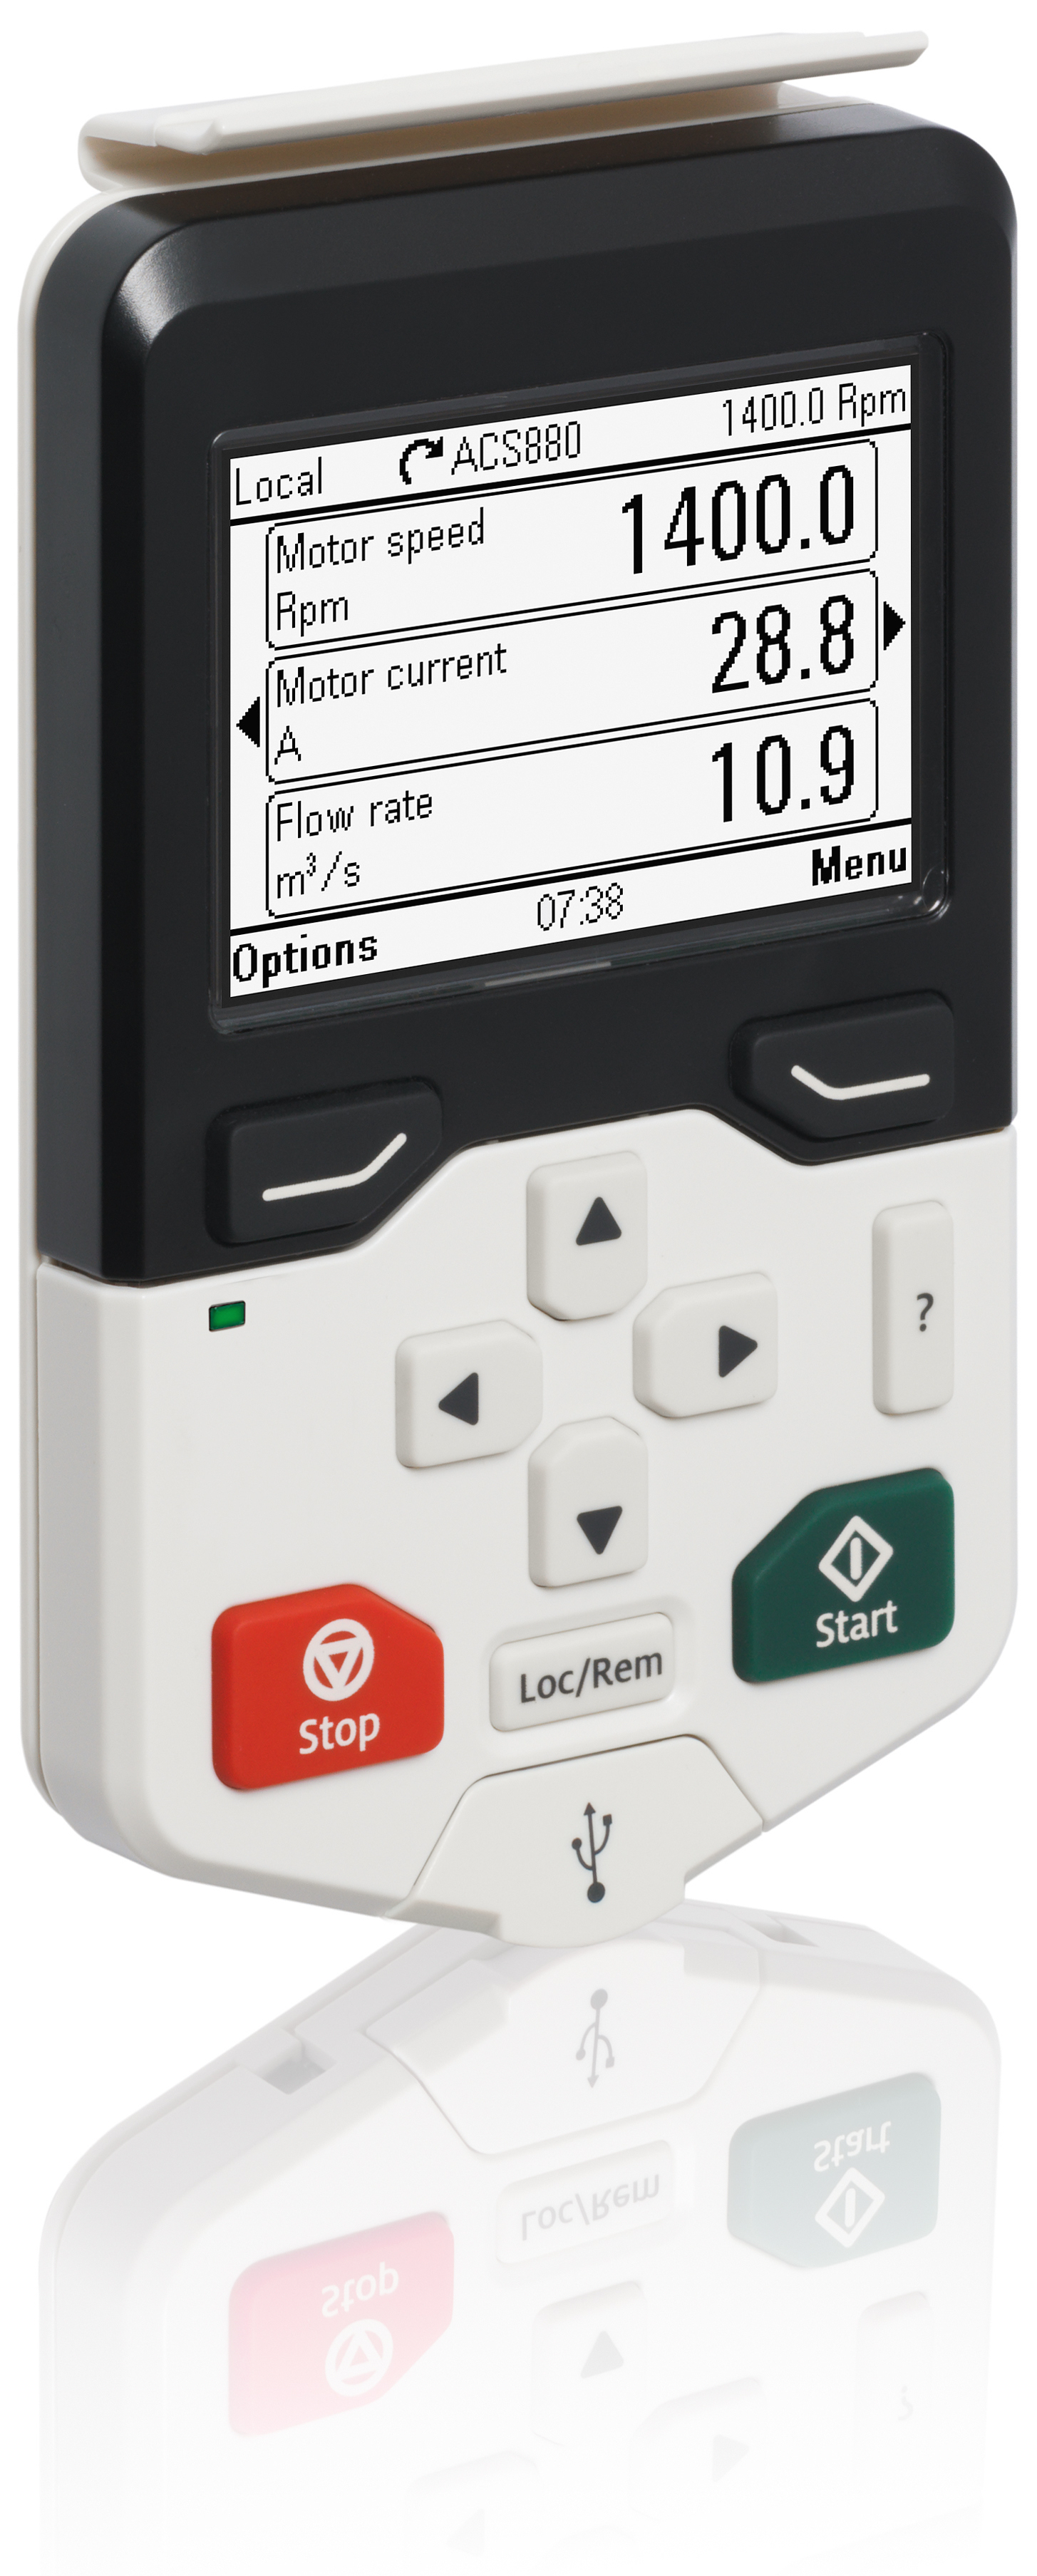
\includegraphics[scale=0.08]{acs880panel}
	\end{center}
	\caption{ABB:n valmistaman ACS880 taajuusmuuttajan ohjauspaneeli.
		\cite{acs880panel}}
	\label{fig:acs880panel}
\end{figure}

\noindent
Toinen tapa taajuusmuuttajan ohjaukseen on I/O. I/O koostuu joukosta analogi- ja digitaalituloja, joilla taajuusmuuttajaa voidaan ohjata esimerkiksi PLC:n avulla. Analogiliitännät käyttävät yleensä standardoitua 4-20mA virtasilmukkaa tai 0-10V jännitesilmukkaa. Digitaalituloissa on käytössä 24V jännitesilmukka, joissa alle 5V jännitetaso tarkoittaa tilaa 0 ja yli 15V tarkoittaa tilaa 1. Taajuusmuuttajan I/O:ssa on lisäksi analogi- ja digitaalilähtöjä, jotka pystytään taajuusmuuttajan sisäistä logiikkaa käyttäen ohjelmoida ohjaamaan järjestelmän muita komponentteja. Nykyään suuremmissa automaatiojärjestelmissä ovat kenttäväylät alkaneet korvaamaan perinteisiä analogi- ja digitaaliliitäntöjä mahdollistaen näin kattavamman ohjauksen ja kustannustehokkaamman järjestelmän.
\\\\
Kenttäväylillä tarkoitetaan joukkoa verkkoprotokollia, jotka on määritelty IEC 61158 -standardissa. Kenttäväylät ovat yleistyneet automaatiossa niiden tuomien kustannussäästöjen ja yksinkertaisuuden vuoksi. Aikaisemmin yleisesti käytössä olleet 4-20mA ja 0-10V analogi- 0-24V digitaalisignaalit mahdollistivat ainoastaan kahden laitteen välisen kommunikoinnin yhtä johdinta käyttäen. Kenttäväyläprotokollat sallivat useiden laitteiden kytkemisen samaan verkkoon. Näin useita signaaleita voi kulkea eri laitteiden välillä samaa johdinta pitkin, jolloin kaapeloinnin tarve vähenee huomattavasti. Nykyään lähes kaikki taajuusmuuttajat sisältävätkin mahdollisuuden kenttäväylän liittämiseen. Yleisesti taajuusmuuttajissa käytettyjä kenttäväyliä ovat esimerkiksi PROFIbus ja ProfiNET. Muita kenttäväyliä voidaan yhdistää käyttäjän tarpeen mukaan erillisten lisäkorttien avulla.
\\\\
Kenttäväylät ovat mahdollistaneet yhä kattavampien automaatiojärjestelmien luomisen. Kenttäväyliä pitkin siirrettävän datan määrä on moninkertainen perinteisiin digitaalisignaaleihin verrattuna. Kenttäväylää hyödyntäviin taajuusmuuttajiin on esimerkiksi mahdollista ohjata etäältä tietokoneelle asennetun ohjelmiston kautta. Tällöin esimerkiksi virheitä voidaan ratkoa ilman, että taajuusmuuttajan luokse täytyy fyysisesti mennä. Tämä voi esimerkiksi kaivoksissa, missä etäisyydet voivat olla kilometriluokkaa, olla merkittävä etu.
\\\\
Yksinkertaisissa sovelluksissa taajuusmuuttajia voidaan myös kytkeä suoraan toisiinsa ilman hintavaa kenttäväyläratkaisua. Tämä tulee kyseeseen esimerkiksi useamman pumpun muodostamissa pumppusysteemeissä, joissa yhden isäntälaitteen ohjaus halutaan saada aikaan kaikissa systeemin taajuusmuuttajissa. Tällöin voidaan käyttää niin sanottua master/slave topologiaa, jossa taajuusmuuttajat ovat kytketty ikään kuin yhdeksi yksiköksi. Tällöin master yksikön ohjaus välittyy suoraan samanlaisena yden tai useamman slave-yksikön ohjaukseksi. Lähes kaikki taajuusmuuttajavalmistajat sallivat master/slave, ratkaisun jotakin omaa kommunikointiväyläänsä hyödyntäen.


%----------TURVALLISUUS------------
\subsection{Turvallisuustoiminnot}
Yhä tiukentuvat turvallisuusmääräykset eri teollisuuden aloilla ovat saaneet taajuusmuuttajavalmistajat kehittämään taajuusmuuttajiin sisäisiä turvallisuustoimintoja. Turvallisuustoiminnoilta vaaditaan erittäin korkeaa luotettavuutta ja ne ovatkin useiden standardien määrittelemiä. Jotta toiminta voidaan hyväksyä viralliseksi standardin määräämäksi turvallisuustoiminnoksi, täyttyy se testata perinpohjaisesti. Turvallisuustoimintojen luotettavuus ilmoitetaan IEC EN 61508 standardin mukaisella SIL-tunnuksella (Safety Integrity Level). SIL kuvaa todennäköisyyttä, jolla turvallisuustoiminto lopettaa toimintansa vaaraa aiheuttaen. SIL1 on tasoista vähiten varma aiheuttaen vaarallisen toiminnon tunnin sisällä 10\textsuperscript{-3}-10\textsuperscript{-5}\% todennäköisyydellä. SIL4 on vastaavasti luotettavin turvallisuustaso aiheuttaen vaarallisen toiminnon seuraavan tunnin sisällä 10\textsuperscript{-6}-10\textsuperscript{-7}\% todennäköisyydellä.[Lähde IEC EN 61508]
%%etsi standardi töissä!
\\\\
Näistä yksinkertaisin ja yleisimmin toteutettu on STO-toiminto (Safe Torque Off). STO on EN 60204-1 -standardin määrittelemä turvallisuustoiminto, joka aktivoituessaan katkaisee moottorin akselille momenttia aiheuttavan sähkövirran. Käytännössä STO on siis hätäpysäytystoiminto, jolla moottori saadaan lopettamaan momentin tuottaminen. STO ei kuitenkaan välttämättä pysäytä moottoria nopeasti, vaan kuormaan kertynyt pyörimismäärä voi pitää kuorman liikkeessä vielä pitkään STO:n kytkeytymisen jälkeenkin. Kuva~\ref{fig:STO} esittää STO-funktion toiminnan kun se kytketään päälle moottorin pyöriessä. STO on erityisen hyödyllinen toiminto, koska hätäpysäytyksen toiminnallisuus pystytään toteuttamaan täysin ohjelmallisesti taajuusmuuttajan sisällä. Tämä poistaa hintavien kontaktorien\footnote{Kontaktori on sähköisesti ohjattava kytkin, joita on perinteisesti käytetty moottorille menevän virran katkaisemiseen.} tarpeen tuoden kustannussäästöjä ja helpottaen asennustyötä.
\begin{figure}[H]
	\begin{center}
	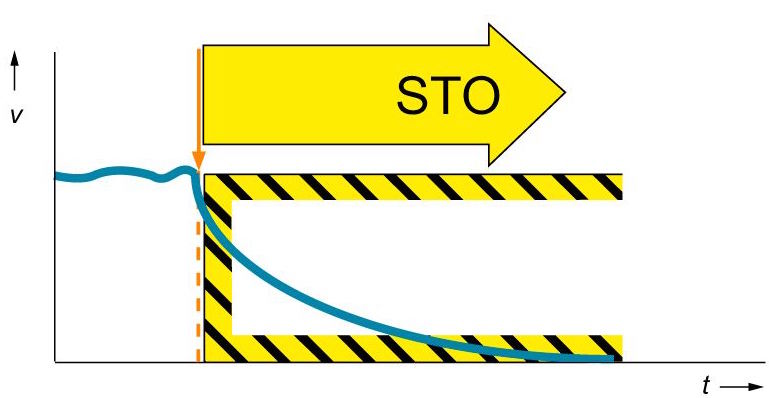
\includegraphics[scale=0.5]{STO}
	\end{center}
	\caption{Moottorin pyörimisnopeus V esitettynä ajan t suhteen STO toiminnon kytkeytyessä.
		\cite{STOkuva}}
	\label{fig:STO}
\end{figure}

\noindent
STO Toiminnon lisäksi EN 60204-1 -standardi määrittelee sarjan muita turvallisuustoimintoja, jotka tekevät kytkeytyessään määritellyn toimintasyklin. Esimerkiksi SS1-toiminto (Safe Stop 1), joka on kuvattu kuvassa ~\ref{fig:SS1}, hidastaa moottorin ramppimaisesti pysähdyksiin ja aktivoi tämän jälkeen STO:n. Nämä toiminnot on yleensä toteutettu taajuusmuuttajaan lisäosana saatavassa turvamoduulissa. Moduuleissa voi olla turvatoiminnot laukaisevien tuloporttien lisäksi rele- tai analogilähtöjä. Lähdöillä pystytään ohjaamaan laitteiston muita turvalaitteita kuten kuormaan kytkettyä mekaanista jarrua, joka voidaan ohjelmoida kytkeytymään samaan aikaan esimerkiksi STO-toiminnon kanssa\cite{FSO}.

\begin{figure}[H]
	\begin{center}
	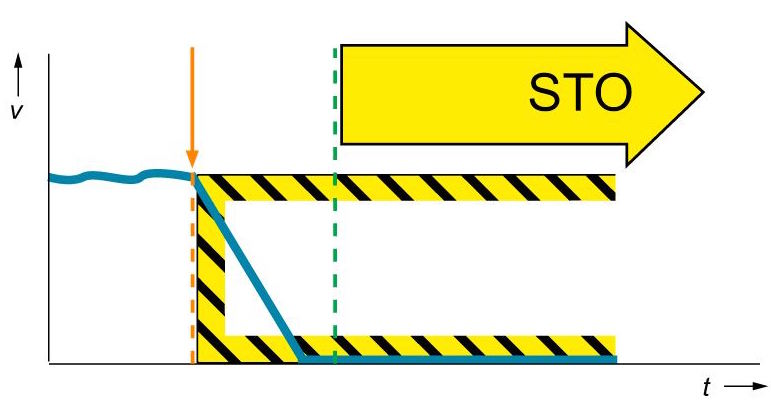
\includegraphics[scale=0.5]{SS1}
	\end{center}
	\caption{Moottorin pyörimisnopeus V esitettynä ajan t suhteen SS1 toiminnon kytkeytyessä.
		\cite{SS1kuva}}
	\label{fig:SS1}
\end{figure}

\noindent
STO ja muiden turvallisuustoimintojen on standardin mukaan oltava eristettyjä järjestelmiä, tarkoittaen että muiden järjestelmien toiminta ei saa vaikuttaa turvallisuustoiminnon toimintaan. Tämä on järkevää turvallisuustoimintojen luotettavuuden kannalta, mutta epätehokasta koska turvasignaalit vaativat oman signaaliväylänsä. Suuressa automaatiojärjestelmässä signaalijohdinten määrä voi kasvaa ongelmalliseksi. Nykyään turvasignaalit onkin mahdollista kuljettaa myös osana kenttäväylän prosessidataa esimerkiksi PROFIsafe kommunikointiteknologiaa käyttäen. PROFIsafea pystytään käyttämään PROFIBUS tai PROFINET kenttäväylän kanssa samassa kenttäväyläkaapelissa. Turvasignaalien yhdistäminen samaan kenttäväylään prosessidatan kanssa vähentää asennus- ja kaapelointikuluja ja yksinkertaistaa automaatiojärjestelmää\cite{MyyntiHaastattelu}. Kenttäväylien yleistyessä prosessiautomaatiossa, myös turvatoiminnot toteutetaan yhä enenemässä määrin kenttäväyliä hyödyntäen\cite{Profisafe}.
\\\\
%%-turvallisuus tärkeää, kaivokset vaarallisia jne.\\
%%-STO, miten voisi hyödyntää?\\
%%-Profisafe yms.

%\subsection{Sovelluskohtaiset ohjelmistot}
%kannattaako tästä tehdä oma kappale?


%väännä rautalangasta mikä on kenttäväylä ja miksi se on hyvä asia. selvennä eroa I/On (miksi tätä voi kutsua prkl!?) ja kenttäväylän välillä.

%mitä etuja tamujen integraatio automaatiojärjestelmään tuo.
%historiaa?
%-Keskitetty automaatiojärjestelmä? 
%-Kenttäväylät?
%Soveluskohtaiset ohjelmistot
% ABBn plc-integraatio edut?  KITTILÄ esimerkki
%Tamujen välinen kommunikointi (yksinkertaiset järjstelmät (pari tamua juttelee keskenään --> ei tarvita kentäväylää ja jäätävää plc:tä))

%oispakaljaa


\subsection{Verkkoon jarruttavat taajuusmuuttajat ja jaettu välipiiri}
Taajuusmuuttajatekniikan kehittyessä ovat yhä monimutkaisemmat taajuusmuuttajajärjestelmät tulleet madollisiksi. Esimerkkeinä näistä tekniikoista ovat nykyään jo yleisesti käytössä olevat verkkoon jarruttavat taajuusmuuttajat ja välipiirin välityksellä toisiinsa kytketyt taajuusmuuttajat. Jotta nämä tekniikat voidaan ymmärtää täytyy tietää perusteet taajuusmuuttajan sisäisestä rakenteesta.
\\\\
Yleisin käytössä oleva taajuusmuuttajarakenne on niin sanottu välipiirillinen taajuusmuuttaja (Voltage-Source Inverter, VSI). Kuvassa~\ref{fig:VSI} nähdään VSI-taajuusmuuttajan kolme pääkomponenttia tasasuuntaaja, välipiiri ja vaihtosuuntaaja. Syöttöverkon vaihtojännite muutetaan ensin tasasuuntaajalla välipiirin tasajännitteeksi ja sitten taas moottorille syötettäväksi vaihtojännitteeksi vaihtosuuntaajalla. Ohjausyksikkö tarkkailee ja säätää kaikkia kolmea komponenttia siten, että ulos tulevan sähkön ominaisuudet ovat halutunlaiset.

\begin{figure}[H]
	\begin{center}
	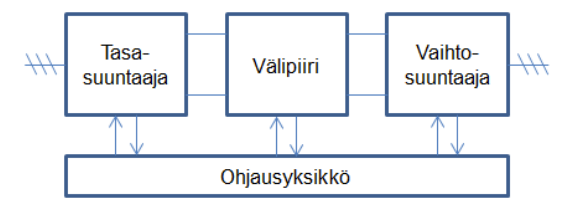
\includegraphics[scale=0.65]{VSI}
	\end{center}
	\caption{Välipiirillisen (VSI) taajuusmuuttajan rakenne.
		\cite[s. 2]{VSI}}
	\label{fig:VSI}
\end{figure}

\noindent
Välipiiriin varastoitu tasajännite toimii energiavarastona vaihtosuuntaajalle, jonka vaatima virta voi vaihdella suuresti kuorman muuttuessa. Useissa sovelluksissa, kuten liukuhihnoissa, tarvitaan useita moottoreita ohjaamaan samaa laitetta. Tällöin on mahdollista, että osa samaan laitteeseen kytketyistä moottoreista on jarruttavassa tilassa ja osa kiihdyttävässä. Kuten aikaisemmin todettiin, jarruttavat taajuusmuuttajat joutuvat purkamaan ylimääräisen energian välipiiristä esimerkiksi jarruvastukseen, jolloin energia menee hukkaan. Yhdistämällä useita taajuusmuuttajia välipiirin välityksellä toisiinsa voidaan vähentää hukkaenergian määrää. Tällöin jarruttavan taajuusmuuttajan luoma ylimääräinen tasavirta pystytään käyttämään toisessa samaan välipiiriin kytketyssä taajuusmuuttajassa moottorin kiihdyttämiseen.
\\\\
Taajuusmuuttajista on myös saatavilla malleja, joita on mahdollista käyttää generaattoreina, eli laitteina, jotka muuttavat kuorman mekaanista energiaa verkon sähköenergiaksi. Tällöin puhutaan niin sanotuista verkkoon jarruttavaista taajuusmuuttajista. Välipiiriin kertyvä ylimääräinen jännite on siis mahdollista purkaa jarruvastuksen sijasta takaisin sähköverkkoon. Ne ovat rakenteeltaan samankaltaisia VSI-tyyppisiin taajuusmuuttajiin verrattuna, mutta tasasuuntaaja on korvattu toisella vaihtosuuntaajalla. Tällöin taajuusmuuttaja kykenee siis ottamaan välipiiristä energiaa kumpaa tahansa vaihtosuuntaajaa käyttäen ja syöttämään sitä moottorille tai sähköverkkoon. Ominaisuus on hyödyllinen esimerkiksi tuotantolaitoksen sisäisessä sähköverkossa, missä laitteet ovat ajoittain kiihdyttävässä ja jarruttavassa liikkeessä. Tällöin hidastuksista aiheutuvaa energiaa ei tarvitse purkaa hukkalämmöksi, vaan se voidaan syöttää takaisin laitoksen sähköverkkoon ja näin käyttää missä tahansa laitoksen prosessissa.



%-miten käytännössä toimii\\
%-Missä voidaan hyödyntää? (hissit, alamäkeen jarrutus, dumppitrukkien sähköraidejärjestelmä, yms.)

\clearpage

%%-------------KAIVOSYMPÄRISTÖN VAATIMUKSET TAAJUUSMUUTTAJILLE----------------
\section{Kaivosympäristön vaatimukset taajuusmuuttajalle}

\subsection{Ympäristöolosuhteet}
Kuten todettu, kaivosympäristö on sähkölaitteille toimintaympäristönä erittäin rasittava \cite[s. 251]{Hakapää}. %% "Kaivoksen olosuhteet ovat raskaimpia, missä sähkölaitteita käyetetään." <-- sitaatiksi?
Sähkölaitteille kaivoksissa rasitusta aiheuttavia tekijöitä ovat
\begin{itemize}
	\item[--] Lämpötila
	\item[--] Kosteus
	\item[--] Ilman epäpuhtaudet
	\item[--] Mekaaniset rasitukset
\end{itemize}
Suurin ympäristön aiheuttama vaara taajuusmuuttajien toiminnalle on ylikuumeneminen ja elektronisten komponenttien vaurioituminen kosteuden, ilman  epäpuhtauksien, mekaanisten iskujen tai tärinän seurauksena. Jotta taajuusmuuttajan luotettava toiminta voidaan taata, täytyy taajuusmuuttajan koteloinnin olla soveltuva käyttöympäristöönsä. Lähes kaikki taajuusmuuttajavalmistajat valmistavatkin taajuusmuuttajia eri suojausluokissa vastaamaan sovellusten vaatimuksia.
\\\\
Euroopassa yleisesti käytössä oleva luokitus sähkölaiteen vesi- ja pölytiiveydelle on kansainvälisen sähköalan standardointitoimiston IEC:n IP-luokitus. Luokitus on kaksiosainen lähtien täysin suojaamattomasta IP00-luokasta ja päätyen täysin vesi- ja pölytiiviiseen IP69-luokitukseen. Liite~\ref{Liite 1} kuvaa eri tasoisten IP-luokitusten mukaiset suojaustasot. Pohjois-Amerikassa on käytössä vastaava NEMA-tiiveysluokitus.
\\\\
Markkinoilla olevat taajuusmuuttajat ulottuvat suojaamattomista IP00-laitteista aina lähes vesitiiviisiin IP66-laitteisiin. IP00 taajuusmuuttajat asennetaan poikkeuksetta ulkoisiin koteloihin, jännitteellisten komponenttien ollessa täysin esillä. IP21 on yleinen käytössä oleva luokka taajuusmuuttajille, jotka tulevat kuivaan tilaan esimerkiksi tehtaan sisälle. Märkiin tai muuten erityistä suojausta vaativiin sovelluksiin tarkoitetut IP66 laitteet kestävät suoran painevesiruiskun kaikista suunnista ja ovat täysin pölysuojattuja. Suuremman suojausluokituksen omaavat laitteet ovat luonnollisesti fyysisesti suurempia ja mekaanisesti haastavampia rakentaa jäähdytyksen ongelmallisuuden vuoksi.
\\\\
Seuraavissa kappaleissa eritellään eri ympäristötekijöiden merkitsevyys kaivosympäristössä. Tarkastelun alla ovat myös vaikutukset mitä näillä olosuhteilla on taajuusmuuttajien toiminnalle sekä miten nämä asiat on otettu huomioon taajuusmuuttajien suunnittelussa. Käsittely koskee pääosin maanalaisia kaivoksia avolouhosten olosuhteiden ollessa tavallista ulkoilmakäyttöä vastaavat. %%such metatext

\subsubsection{Lämpö}
%%-Kaivosten lämpötilat
%%-Laitteiden käyttölämpötilat, derating
%%-Jäähdytysratkaisut(neste,kanava,perinteinen,cold plate,...)
Maanalaisissa kaivoksissa lämpöolosuhteet eroavat huomattavasti maanpäällisistä. Kaivoksessa lämpöä aiheuttaa itse kallioperän lämpö, ilman puristuminen, lämpimät pohjavesivuodot, koneet, valaistus ja räjäytykset\cite[s.305]{Hakapää}. 
\\\\
Etenkin syvissä kaivoksissa kallioperän lämpö on suurimpia kaivoksen sisäilman lämmittäjiä. Kallioperän lämpötila kasvaa syvemmälle mentäessä noin 25-30\textdegree C/km, joten jo kilometrin syvyisessä kaivoksessa lämpötila voi yltää 30-40\textdegree C riippuen paikallisesta ilmastosta \cite[s. 62]{maanlampo}. %% s.62: maan lämpeneminen/km 
Esimerkkinä todettakoon Suomen syvin metallikaivos Pyhäsalmella on 1400 metriä syvä, jolloin lämpötila ilman ilmanvaihtoa kohoaa yli kolmeenkymmeneen asteeseen. Hyvin suunnitellussa kaivoksessa kuitenkaan harvoin on ongelmana, että kaivoksen sisälämpötila olisi liian korkea laitteiden toiminnalle. Olennaista on, että lämpö pystytään johtamaan ulos sitä tuottavista laitteista ja ilmaa lämmittävästä kallioperästä jotta lämpötila pysyy koneille ja henkilöstölle edullisena. Ilmanvaihtojärjestelmän suunnittelun tärkeys tulee tässä vahvasti esille. Taajuusmuuttajien käyttöä osana kaivoksen ilmanvaihtojärjestelmää käsitellään tarkemmin luvussa \textit{4.2.5 Tuulettimet ja ilmanvaihto}. Kaivoksen lämpötilan noustessa esimerkiksi tuuletusjärjestelmän häiriön takia taajuusmuuttajien sisäinen lämpötilan tarkkailu osaa automaattisesti alentaa tuotettua sähkövirtaa ja näin komponenteissa syntyvää lämpömäärää. Tämä estää laitteen vioittumisen ylikuumenemisen takia.
\\\\
Taajuusmuuttajat ovat hyvin energiatehokkaita laitteita siirtäen noin 98\% vastaanottamastaan energiasta moottorille\cite{ABBinmining}. Energiasta 2\% kuitenkin muuttuu taajuusmuuttajan sisäisenä häviönä lämpöenergiaksi. Tämä tarkoittaa esimerkiksi 500kW taajuusmuuttajan vaativan noin 10kW jäähdytystehon toimiakseen jatkuvasti. Tämä lämpöenergia poistetaan taajuusmuuttajasta ilma- tai nestejäähdytyksen avulla ympäristöön.
 
%%derating ja muut suojat????

\subsubsection{Kosteus}
%%-Kaivosten kosteus, sumu, kaapelit vesitiiviitä
%%-Laitteiden kosteuskestävyys?
%%-IP ja - NEMA-luokitukset?
Kosteus ilmenee kaivoksissa kahtena ilmiönä: ilmankosteutena ja nestemäisenä vetenä. Suurimman uhan sähkölaitteen toiminnalle aiheuttaa nestemäinen vesi, jota kondensoituu kosteasta ilmasta. Kaivoksissa suhteellinen ilmankosteus saattaa nousta hyvinkin korkeaksi suljetun tilan sitoessa kostean ilmamassan.  Syvimmissä kaivoksissa voidaan saavuttaa jopa yli 95\% suhteellinen ilmankosteus \cite{manchao}. Kondensoituvan veden lisäksi kaivoksissa täytyy ottaa huomion myös katosta mahdollisesti tihkuva vesi.
\\\\
Kaivoksen tekniikkaa suunniteltaessa on otettava huomioon sähkölaitteiden kosteudensieto ja sijoitettava laitteet joko eristettyyn sähkötilaan tai hankkia ne riittävällä suojausluokituksella varustettuna. Ilmajäähdytteisten laitteiden haasteena on yleisesti niiden pienempi IP-luokitus, mikä sallii veden kondensoitumisen laitteen sisälle\cite{Pallasmaa}. Vesijäähdytys tarjoaa yleisesti paremman tiiveysluokituksen, sillä laitetta viilentää ilman sijasta suljettu nestejärjestelmä, jolloin ilmalla ei ole lainkaan pääsyä kosketuksiin elektroniikan kanssa. Kaivoksen tilapäisen luonteen vuoksi nestejärjestelmät voivat kuitenkin osoittautua epäkannattaviksi.
\\\\
Jotta myös ilmajäähdytteisiä laitteita pystytään käyttämään vaativissa olosuhteissa täytyy korkeamman suojausluokan laitteissa jäähdytysilma johtaa laitteen läpi sen pääsemättä kosketuksiin elektroniikan kanssa. Tämä on usein toteutettu jakamalla laite sisäisesti kahteen osaan: kosteudelle herkän elektroniikan sisältävään ilmalta eristettyyn osioon ja jäähdytysosioon, jossa jäähdytyselementti  sijaitsee.  Lämpö johtuu komponenteista jäähdytyselementin säleikköön, josta se johtuu säleikön läpi kulkevaan ilmaan. Ilma kierrätetään laitteen läpi tuulettimilla, joiden täytyy kestää ympäristön olosuhteet. Tuuletin onkin yksi ilmajäähdytteisen taajuusmuuttajan herkimmin hajoavia komponentteja \cite{Muttilainen}. Kuva~\ref{fig:IP55} esittää IP55 luokitellun taajuusmuuttajan, jossa jäähdytysilma ohjataan jäähdytyselementin kautta sen pääsemättä kosketuksiin elektroniikan kanssa.

\begin{figure}[H]
	\begin{center}
	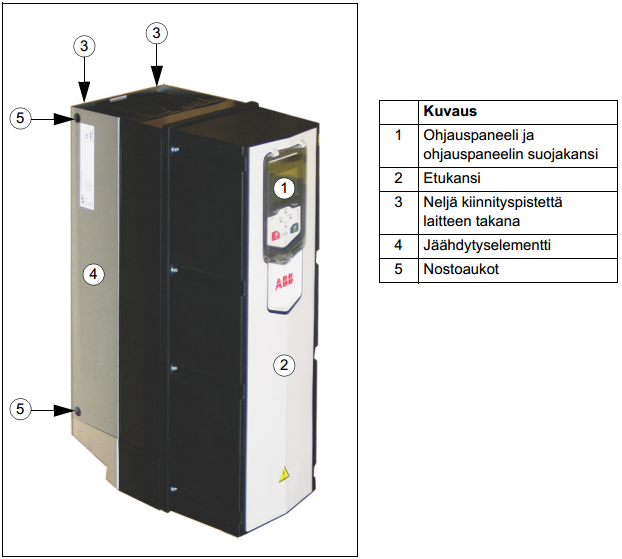
\includegraphics[scale=0.9]{IP55}
	\end{center}
	\caption{ACS880-01 taajuusmuuttaja IP55-koteloinnilla
		\cite[s.28]{880hwman}}
	\label{fig:IP55}
\end{figure}

\noindent
Toinen mahdollisuus on sijoittaa jäähdytyselementti laitteen ulkopuolelle, jolloin yleisesti puhutaan niin sanotusta laippa-asennuksesta (flange-installation). Tällä tekniikalla taajuusmuuttaja pysytään upottamaan ulkoiseen koteloon ja kierrättämään jäähdytysilma kotelon ulkopuolella esimerkiksi tuuletuskanavassa. Tämä eristää taajuusmuuttajan täysin tuuletusilmasta ja sallii tehokkaan lämmön poistamisen tuuletuskanavan välityksellä. Kuvassa 2 esitetään hahmotelma laippa-asennetusta taajuusmuuttajasta, jossa jäähdytyselementti on eristetty omaan tilaansa.

\begin{figure}[H]
	\begin{center}
	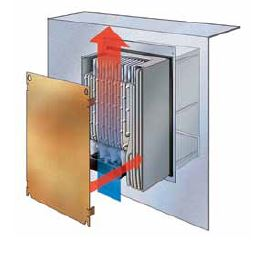
\includegraphics{flange}
	\end{center}
	\caption{Hahmotelma laippa-asennetusta taajuusmuuttajasta
		\cite[s.6]{danfoss}}
	\label{fig:flange}
\end{figure}

\noindent
Kaivoksen kiinteissä asennuksissa on mahdollista rakentaa myös kokonaisia kosteuden- ja pölynkestäviä sähköhuoneita, joissa pystytään käyttämään normaalin IP21 tai IP20 tiiveysluokituksen omaavia sähkölaitteita \cite[s.253]{Hakapää}. Taajuusmuuttajien sijoittelu näihin pysyviin rakennelmiin voi kuitenkin olla kannattamatonta moottorikaapelien pituuksien kasvaessa kohtuuttoman pitkiksi.





%%Pallasmaa Aaro selvitä dippatyö: ulkokäyyttöön suunnitellun tehoelektroniikkalaitteen konseptisuunnittelu.

%%ACS880-01 HW manual, kuvat tuuletuskanavista ja laitteesta!!
%%ACS880-01 Flange-manual lähteeksi?

%%Kysy petriltä EMC-häiriöistä!
%% flangen ip-luokka?

%%ota mallia dippa: Lifetime and reliabilty of .... fan	

\subsubsection{Pienpartikkelit}
%%-Pöly\\
%%-Kemikaalit\\
%%-Syövyttävyys\\
%%-Elektroniikan eristys (flange)
Kaivoksen ilmassa on kosteuden lisäksi pölyä ja muita kemikaaleja, joita muodostuu työkoneiden toiminnan ja räjäytysten seurauksena. Samoista seikoista johtuen myös hiekkaa voi kulkeutua kosketuksiin sähkölaitteiden kanssa. Hiekkaa ja pölyä esiintyy kaikissa ulkoympäristöissä, mutta niiden laatu haitallisuus sähkölaitteiden toiminnalle määräytyy paljolti ympäröivän kosteuden ja maaperän laadun seurauksena. Kaivosympäristössä pölyn joukossa on kaivoksen luonteesta riippuen vaihtelevat määrät yhdisteitä, jotka kosteuden kanssa voivat aiheuttaa korroosiota.
\\\\
Korroosio on tietyissä olosuhteissa merkittävä sähkölaitteita rasittava tekijä. Korroosiota tapahtuu varuksellisen hiukkasen joutuessa kosketuksiin sähkölaitteen metallisen pinnan kanssa elektrolyytin, esimerkiksi veden, välityksellä. Voimakas korroosiota aiheuttava ioni on esimerkiksi kloridi (Cl\textsuperscript{-}), jota esiintyy kaikissa suolaisissa ympäristöissä. Lisäksi voimakkaasti korrosoivia ioneja ovat myös dieselkoneiden pakokaasuista vapautuvat rikin (SO\textsuperscript{x}) ja typen oksidit(NO\textsuperscript{x}). Sähkölaitetta suunniteltaessa käyttöympäristön mahdolliset korroosiovaikutukset täytyy ottaa huomioon laitteen materiaalivalinnoissa. Esimerkiksi muovit ja alumiini ovat korroosionkestoltaan hyviä materiaaleja ja ovatkin yleisesti käytössä taajuusmuuttajien kuorissa.
\\\\
Korroosion lisäksi pöly ja hiekka voivat aiheuttaa sähkölaitteen ylikuumenemisen tai sähkövian. Pölyisissä ympäristöissä on pidettävä huoli että pöly ja muu hienorakeinen aines kuten hiekka ei pääse tukkimaan sähkölaitteiden mekaanisia tai sähköisiä osia. Yleisin pölyn aiheuttama ongelma lienee ilmajäähdytteisen sähkölaitteen jäähdytyselementin peittyminen pölyllä ja muilla epäpuhtauksilla alentaen jäähdytyselementin lämmönsiirtokykyä. Ilman epäpuhtaudet voivat vaikuttaa haitallisesti myös ilmaa jäähdytyselementin läpi puhaltavaan puhaltimeen, mikä voi pahimmassa tapauksessa estää puhaltimen toiminnan.\cite{Pallasmaa}
%%miten estetään (putsaus ym. materiaalivalinnat IP9001 puhallin)
\\\\
Hienorakeinen pöly voi helposti kulkeutua kosketuksiin myös sähkölaitteen elektronisten osien kanssa. Yhdistettynä kosteuden kanssa elektroniikan päälle kertynyt pöly voi muuttua johtavaksi aiheuttaen pahimmassa tapauksessa vuotovirtoja tai läpilyönnin. \cite{Pallasmaa} Pölyn ja muiden hiukkasten aiheuttamien sähkö-, lämpö, ja korroosio-ongelmien takia on tärkeää huolehtia sähkölaitteiden asianmukaisesta huollosta. Sähkölaitteen kotelo tulisi säännöllisesti puhdistaa kertyneestä liasta ja tarkistaa ettei korroosiota ole päässyt syntymään. Kaivossuunnittelussa tulisi ottaa huomioon kaivoksen ilmanlaatu ja mitoittaa laitteiden suojausluokitus sitä vastaavaksi. Vaihtoehtoisesti voidaan käyttää muita tapoja kuten ulkoista sähköhuonetta tai aikaisemmin mainittua laippa-asennusta.

%-kiviainesta
%-räjähteitä
%-Mitä aiheuttaa?
%-tuulettimet tukkeutuu
%-vesi + paska = korroosio
%-elektroniikan yhteydessä läpilyöntejä

\subsubsection{Mekaaniset rasitukset}
Sähkölaitteet voivat kuljetuksen, asennuksen ja käytön aikana altistua tärinälle ja iskuille. Tärinä ja iskut rasittavat laitteen komponentteja lyhentäen sen elinikää. Turvatakseen toimintansa ovat useat taajuusmuuttajavalmistajat määritelleet suurimmat tärinän ja iskujen arvot, joita taajuusmuuttaja luotettavasti kestää. IEC 60082-2 standardi määrittelee tavat sähkölaitteiden tärinän- ja iskunkeston mittaamiselle. Standardissa tärinä ilmaistaan sen amplitudin, taajuuden ja kiihtyvyyden summana ja iskut kiihtyvyytenä.\cite{IEC60082-2}
%%IEC:standardit (ACS880HWmanual s.174)
\\\\
Kaivosympäristössä taajuusmuuttajaan kohdistuvat mekaaniset rasitukset riippuvat paljolti laitteen asennuspaikasta. Kaivoksen kiinteissä järjestelmissä kuten ilmanvaihdossa taajuusmuuttajat on tyypillisesti asennettu seinälle tai lattialle sähkötiloihin. Suuremmissa laitteissa kuten murskaimissa ja työkoneissa taajuusmuuttajat ovat asennettuna osaksi koneen rakennetta ja liikkuvat koneen mukana altistuen täten vaihteleville olosuhteille.
\\\\
Kaivoksen kiinteät taajuusmuuttajat on tyypillisesti asennettu eristettyyn sähkötilaan. Jos kaivoksessa louhitaan malmia käyttäen räjähteitä täytyy laitteiden sijoittelussa ottaa huomioon etäisyys räjäytyspaikkaan tärinän kulkeutuessa kallioperässä pitkiäkin matkoja. Jos laitteita ei pystytä sijoittamaan tarpeeksi kauas, voidaan käyttää tärinänvaimentimia, jotka asennetaan taajuusmuuttajan ja asennuskohteen väliin. Tärinänvaimentimet muuttavat tärinän liike-energian kitkan avulla lämmöksi. Kumi on tyypillinen tärinänvaimentimissa käytetty materiaali sen elastisten ominaisuuksien vuoksi.
\\\\
Hyvin tärinäsuojatun taajuusmuuttajan suurimmat mekaaniset rasitukset aiheutuvat kuljetuksesta ja asennuksesta. Vaikkakin mahdollista, on laitteen vaurioituminen kuljetuksen tai asennuksen aikana epätodennäköistä. Sijoitetun pääoman suuruudesta johtuen kaivosteollisuuden taajuusmuuttajat asennetaan pääosin ammattilaisten toimesta. Kestävällä pakkauksella voidaan varmistaa laitteen päätyminen ehjänä sovelluskohteeseen saakka.
\\\\ 
Työkoneisiin kuten murskaimiin asennetut taajuusmuuttajat altistuvat vaihtelevalle tärinälle laitteen sovelluskohteesta riippuen. Kiinteästä asennuksesta poiketen työkoneissa voi esiintyä jatkuvaa jaksollista tärinää mikä voi aiheuttaa resonointia\footnote{resonanssi on ebin} laitteen komponenteissa. Haitallisen resonanssin kannalta olennaisimpia ovat matalat värähtelytaajuudet, jotka aiheuttavat suurimmat siirtymät ja siten myös jännitykset sähkölaitteen komponenteissa.[Lähde]. Laitteen kuori ja komponentit tulisi suunnitella siten, että matalia resonanssitaajuuksia ei olisi käytettävän moottorin käyttöalueella.[Lähde?]
%% Viite: Vibration analysis for electronic equipment (pääkirjasto)
%%Taajusmuuttajien käyttö tuulivoimaloissa <--- hyviä lähteitä tähän

\subsection{Kaivoksen sähköverkko}
Kaivokset ovat suuria sähkönkuluttajia. Kaivosalueella sähköä kuluttavat itse kaivanto, rikastamo, toimistotilat ja joskus myös asuinrakennukset. Jos sähkö tilataan ulkoiselta toimittajalta, toimitetaan se yleensä 110kV suurjännitelinjaa pitkin ja muunnetaan kaivosalueella jakelujännitteeksi. Suomessa suurin sallittu jakeluverkon jännite on 20kV. Suuren jakelujännitteen etuna ovat pienemmät häviöt pitkillä etäisyyksillä ja mahdollisuus käyttää poikkipinta-alaltaan pienempiä siirtokaapeleita. \cite[s. 251-253]{Hakapää}
\\\\
Jakelujännite muunnetaan edelleen käyttöjännitteeksi jakelumuuntajilla. Kaivosalueilla on yleisesti käytössä 400V:n kolmivaihejärjestelmä. 400V järjestelmän etuna, en että tavallista 230V vaihtovirtaa saadaan suoraan samasta järjestelmästä yhden vaihe- ja nollajohtimen väliltä. Toinen standardisoitu jännite on 690V käyttöjännite, jota käytettäessä päästään pitempiin kaapelietäisyyksiin tai pienempiin poikkipinta-aloihin. \cite[s. 251-253]{Hakapää}
\\\\
Joissakin tapauksissa voi myös olla kannattavaa tuottaa kaivosalueen tarvitsema sähköenergia paikanpäällä. Syrjäisillä alueilla vai olla mahdollista että tarpeeksi vahvaa verkkoa ei ole saatavilla tai että verkkoa ei ole ollenkaan. Tämä tulee harvoin kysymykseen Suomessa vahvan ja kattavan sähköverkon ansiosta. Myös sähköverkon luotettavuus pitää olla korkea. Jos katkokset sähkönjakelussa ovat alueella yleisiä voi voimantuotanto paikanpäällä olla kannattavampi vaihtoehto suuremmista kustannuksista huolimatta. Voimantuotanto paikanpäällä toteutetaan yleensä dieselvoimalaitoksella, jossa dieselmoottorit tuottavat sähköenergiaa generaattoreiden välityksellä. Kompromissi näiden kahden väliltä on varavoimalaitos, joka tuottaa vaaditun energian paikanpäällä sähkökatkoksen aikana. \cite[s. 251-253]{Hakapää}
\\\\
Ilman taajuusmuuttajaa ohjatut sähkömoottorit vaativat käynnistyksessä moninkertaisen virran normaaliajoon verrattuna. Tämä voi heikon kantaverkon alueella muodostua ongelmaksi suurten sähkömoottoreiden aiheuttaessa käynnistyksessä suuren heilahduksen sähköverkon virtaan. Taajuusmuuttajalla ohjattu moottori ottaa verkosta kohtuullisen tasaista virtaa, jolloin suuria verkon heilahteluita ei pääse muodostumaan. Tämä voi muodostua kynnyskysymykseksi alueilla, joissa siirtoverkko ei kestä suuria virtapiikkejä. \cite{MyyntiHaastattelu}

%%Kaivoksen sähköverkko (EMC häiriöt)\\
%%-jännite,laajuus, häiriönsieto, EMC\\
%%-kuristimien/filttereiden tarpeellisuus

\subsection{Käyttöikä ja luotettavuus}
Luonteestaan johtuen kaivokset ovat tilapäisiä rakennelmia eliniän riippuessa monista seikoista kuten esiintymän suuruudesta, esiintymän syvyydestä ja louhittavan malmin markkinahinnan kehityksestä. Rajatusta käyttöajasta ja suuresta alkuinvestoinnista johtuen laitteiden halutaan ensiasennuksen jälkeen lähtökohtaisesti toimivan koko kaivoksen elinkaaren ajan. Toisin sanoen luotettavaksi osoittautuneita järjestelmiä harvoin lähdetään vaihtamaan kesken kaivoksen toiminnan vaikka uusia mahdollisesti parempia olisi saatavilla. Tässä korostuvat asiakkaan kokemukset taajuusmuuttajien luotettavuudesta. Teknisesti kehittyneempi ratkaisu voi hävitä tarjouskilpailun asiakkaan kokemusten perusteella luotettavammalle laitteelle. \cite{MyyntiHaastattelu}
\\\\
Kaivosteollisuuden vaatiman huomattavan suuren alkuinvestoinnin seurauksena lähes kaikki kaivosteollisuuden toimijat ovat suurikokoisia yrityksiä, joilla on näin resurssit suunnitella kaivostensa automaatiojärjestelmä itse aina logiikkaohjainten (PLC, Programmable Logic Controller) ohjelmistoja myöten. Yrityksen oman logiikkasuunnittelun ansiosta taajuusmuuttajan sisäisen älyn tarve vähenee. Oman automaatiojärjestelmän käyttö on yrityksen kannalta järkevää, sillä korjaus ja päivitys voidaan näin hoitaa oman henkilöstön avulla ilman tarvetta ulkoisille toimijoille. \cite{MyyntiHaastattelu}
\\\\
Kaivostoiminnassa käyttökatkot eli kaivostoiminnan pysähtyminen tai hidastuminen tietyn järjestelmän komponentin kuten taajuusmuuttajan rikkoutumisen seurauksena on merkittävä kaivoksen kannattavuuteen vaikuttava tekijä kiinteiden kulujen ollessa suuret tuotannon määrästä huolimatta. Lisäksi taajuusmuuttajia käytetään turvallisuuden kannalta kriittisissä toiminnoissa kuten ilmanvaihdossa. Tämän takia taajuusmuuttajilta edellytetään ensisijaisesti korkeaa luotettavuutta ja hyviä tukitoimintoja.\cite{MyyntiHaastattelu}
%%Viitteet jotenkin järkevämmin???


%% Tähän voisi kirjoittaa suuret toimittajat: luotettavuus, robustisuus > hienot ominaisuudet (tekevät omat settinsä PLC:n avulla, eivät halua ulkoisten kikkailuja --> oma henkilöstö osaa käyttää ja korjata).
%%servicen rooli? suuri toimittaja --> globaali ja nopea huolto (isot tekijät huoltavat itse?)

%%Hinta tärkeinä tähän vai vasta yhteenvetoon?





\clearpage


\section{Taajuusmuuttajien sovellukset kaivoksissa}
Kaivosteollisuus käsittää laajan joukon aliprosesseja, joissa kussakin käytetään siihen suunniteltuja koneita. Näitä kaivosalueella tapahtuvia malmin rikastamisen välivaiheita ovat louhiminen räjäyttämällä tai poraamalla, louheen siirto, murskaus ja rikastus. Kuvassa~\ref{fig:Kaivosprosessi} nähdään kaivosprosessin päävaiheet. Polttoaineen hinnan kasvaessa kaivoksissa on siirrytty pääosin sähköä voimanaan käyttäviin koneisiin, mikä on luonut tarpeen sähkömoottorien tehokkaalle ohjaukselle taajuusmuuttajilla. Nykyään dieselkoneita käytetään lähinnä vain liikkuvassa kalustossa, mihin sähkönsiirto johdinta pitkin tai akuston avulla voi olla hankalaa tai epäkannattavaa.
\\\\ 
%Mitä kaikkea tapahtuu (louhinta,murskaus, rikastus, siirto, ym). Sähkönkäyttö. Teollisuuden laajuus, kehittyminen, automaation taso

\begin{figure}[H]
	\begin{center}
	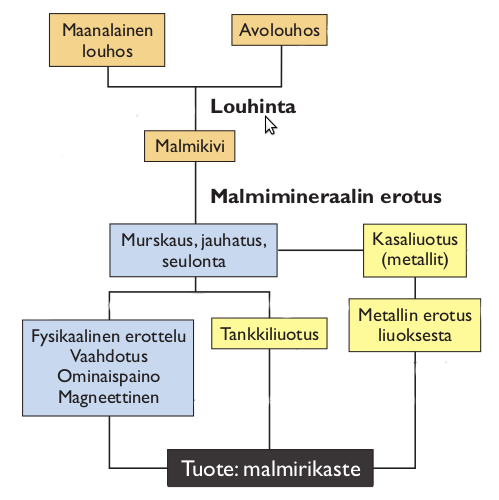
\includegraphics{Kaivosprosessi}
	\end{center}
	\caption{Kaivosprosessin päävaiheet.
		\cite{Kaivosprosessi}}
	\label{fig:Kaivosprosessi}
	
\end{figure}
\noindent
Louhe saadaan irti maaperästä räjäyttämällä tai louhimalla. Louhinnassa voidaan käyttää useita eri menetelmiä, mitkä riippuvat paljolti maaperän laadusta ja louhittavasta mineraalista. Irroitettu louhe täytyy ennen rikastusprosessia hienontaa murskaamalla. Murskaus tapahtuu yleensä kahdessa tai kolmessa osassa, esi-,väli- ja hienomurskauksessa, jossa kussakin raekoko pienenee noin kuudennekseen alkuperäisestä \cite[s. 198]{Hakapää}. Esimurskaus voidaan suorittaa jo kaivoksen sisällä, jolloin murskattu malmi on helppo siirtää kaivoksesta esimerkiksi kuljetinta käyttäen. Suurirakeinen malmi täytyy kuljetttaa dumppereilla eli kaivoskäyttöön suunnitelluilla siirtokoneilla murskattavaksi. 
\\\\
Murskauksessa louhe murskataan pienempään muotoon puristamalla tai iskemällä. Louhe syötetään murskaimeen syöttimellä, jonka tyyppi riippuu siirrettävän louheen luonteesta. Ennen murskaimia louhe voidaan syöttää seulaan joka erottelee suuren ja pienen aineksen toisistaan niin, ettei seuraavaan murskausvaiheeseen päädy tarpeettomasti sille liian pientä ainesta. Hienonnusprosessin jälkeen malmi rikastetaan. Rikastuksessa malmista erotetaan tarpeeton sivuaines, jotta halutun mineraalin pitoisuus nousee. Tämä voidaan tehdä malmista riippuen usealla tavalla. \cite[s. 197-199]{Hakapää}
\\\\
Tämä kappale käsittelee mainittujen prosessivaiheiden suorittamiseen tarvittavien laitteiden toimintaa. Tarkastelun alla ovat koneet, joissa erityisesti käytetään taajuusmuuttajia tai niille olisi potentiaalisia käyttömahdollisuuksia. Tarkastelussa on myös taajuusmuuttajien yleinen teholuokka kyseisissä sovelluksissa ja niiden sijoittelu kaivosympäristöön.


\subsection{Taajuusmuuttajien kokoluokat ja sijoittelu}
-5.12 Excu Metsolle Tampereelle. Sieltä tietoa tähän

-Teho- ja jänniteluokat (kuvia!)\\
-Seinä,lattia,floorstanding\\
-Asennuspaikat\\
-fyysinen koko?\\
-Hyvät/huonot puolet\\
-kaapelien pituus, EMC\\
-Kommunikointi (kenttäväylät, analogisignaalit)\\

\subsection{Sovellukset}

\subsubsection{Kaivoskoneet}
Kaivoksissa käytetään joukkoa erilaisia liikkuvia työkoneita. Niitä käytetään pääasiassa räjähteiden asentamiseen ja poraamiseen sekä malmin liikuttamiseen ja käsittelyyn. Näitä ovat esimerkiksi kaivinkoneet, louhosautot, kauhakuormaajat, porausvaunut ja LHD:t (Load Haul Dump)\footnote{"LHD:t ovat tehokkaita ja suurikauhaisia lastauskoneita, jotka on suunniteltu työskentelemään maanalaisissa kaivoksissa ja ahtaissa tiloissa." \cite[s. 192]{Hakapää}}. Sähkökäyttöisten ajoneuvojen käyttö on yleistynyt kaivoksissa polttoainekustannusten noustessa ja sähkövoimatekniikan kehittyessä. Myös dieseliä ja sähköä vuorotellen käyttäviä hybridiajoneuvoja esiintyy \cite{Brown}.
\\\\
Liikkuvissa ajoneuvoissa taajuusmuuttajien käyttökohde on yleisimmin laitteen liikkumiseen käytettyihin pyöriin liitetyn sähkömoottorin ohjaaminen. Liikkuvissa koneissa hyötysuhde ja liitettävyys sähköverkkoon ovat taajuusmuuttajien suurimmat edut verrattuna perinteiseen polttoainemoottoriin \cite{Brown}. Taajuusmuuttajilla vaihtovirtasähkömoottoria pystytään ajamaan jatkuvasti sen optimialueella toisin kuin polttomoottoreissa, joissa paras hyötysuhde saavutetaan vain tietyllä kierrosalueella \cite{Brown}. Myös esimerkiksi moottorista erillinen jäähdytysjärjestelmä säästää energiaa kun jäähdytyspuhaltimia ei tarvitse tarpeettomasti pyörittää moottorin tahdissa kuten polttomoottorikoneissa \cite{Brown}. 
\\\\
Sähköverkkoon liitettävyydellä tarkoitetaan kaivoskoneen kytkemistä osaksi kaivoksen sähköverkkoa niin että kone saa käyttövoimansa suoraan verkosta. Tällöin liikkuvassa koneessa on  esimerkiksi kaapelikela, joka koneen liikkuessa syöttää sähköjohdinta koneen taakse ja vastaavasti kerää sen takaisin koneen peruuttaessa. Tämä luonnollisesti rajoittaa koneen liikealuetta, mutta on käyttökelpoinen esimerkiksi LHD-koneiden (kuvassa~\ref{fig:LHD}) kanssa niiden valmiiksi rajoittuneesta työympäristöstä johtuen. Toinen yleisesti dumpperien eli suurten louhosautojen kanssa käytettävä liitäntäratkaisu on kannatinjohto \cite{Brown}. Kannatinjohto on ripustettuna dumpperien ajoväylän yläpuolelle ja dumpperit kytkeytyvät siihen junien tapaan koskettimella. Sähköverkkoon kytketyt kaivoskoneet tuovat energiansäästön isäksi muita etuja etenkin maanalaisissa kaivoksissa. Maanalaisissa kaivoksissa dieselkoneiden käyttö luo pakokaasupäästöjä ja huomattavat määrät lämpöä, joka täytyy tuulettaa ulos. Sähkökäyttöisissä koneissa hiukkapäästöjä ei ole ja korkean hyötysuhteen ansiosta hukkalämmön määrä on mitätön.
\\\\
\begin{figure}[H]
	\begin{center}
	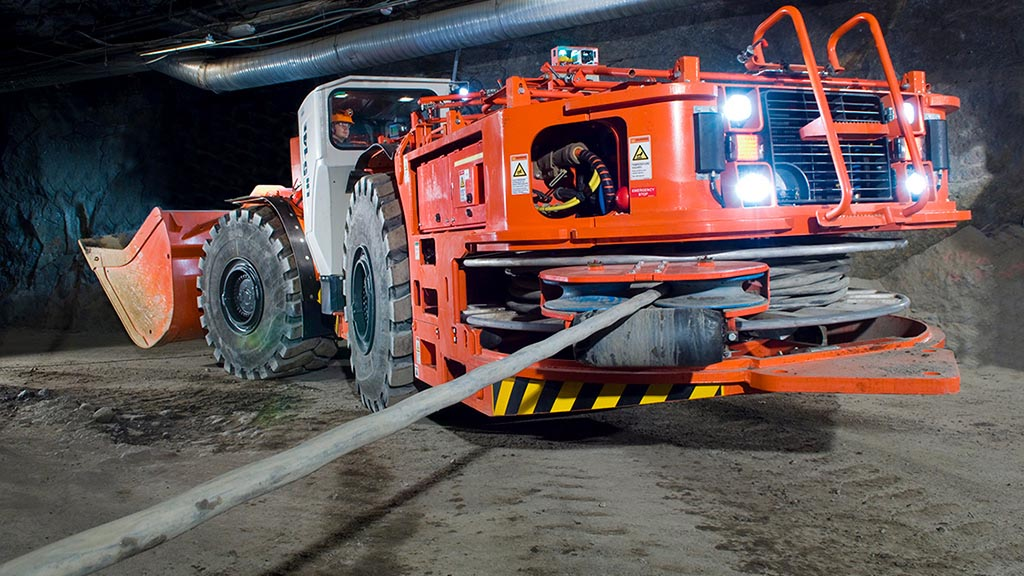
\includegraphics[scale=0.35]{LHD}
	\end{center}
	\caption{Sähkökäyttöinen LHD.
		\cite{LHD}}
	\label{fig:LHD}
\end{figure}
\noindent
Suunniteltaessa taajuusmuuttajia kaivoskoneisiin, täytyy ottaa huomioon useita seikkoja. Taajuusmuuttajat joutuvat koneen osana erittäin rankoille ympäristöoloille ja tärinälle, joten vankka ja tiivis kotelointi on tärkeä. Samalla tarvittavasta jäähdytyksestä on huolehdittava esimerkiksi erottamalla jäähdytysrivasto elektroniikasta. Kaivoskoneet on yleensä rakennettu myös hyvin kompakteiksi maksimoiden kuormattavan massan. Tämä asettaa vaatimukset taajuusmuuttajien fyysiselle koolle ja tehotiheydelle.
%-mitä erilaisia? (jäätävän isot osana sähköverkkoa vs pienet)\\
%-Multidrive ohjaamaan kaikkea?
%-Sähködumpperit maanalaisissa kaivoksissa (koneenrakentajat haluu tamui!)
%-Isot dumpperit ja sähköraide
%-täryttimet/suotimet?

\subsubsection{Kuljettimet}
Kuljettimet ovat yleinen ratkaisu kaivoksissa murskatun malmin kuljettamiseen paikasta toiseen. Yleisin käytetty kuljetintyyppi on hihnakuljetin, jossa kannatusrullaston päällä kulkee tekstiili- tai vaijerivahvisteinen hihna. Hihnaa liikuttaa hihnaston toisessa päässä oleva vetorumpu, jonka akselille on kytketty sitä pyörittävä sähkömoottori. Toisessa päässä sijaitsee kääntörulla, jonka on yleensä vapaasti pyörivä. Kuva~\ref{fig:hihnakuljetin_rakenne} esittää perinteisen hihnakuljettimen suurpiirteisen rakenteen. Hihnan kireyttä säädetään ruuvikirityslaitteella, jolla rumpujen etäisyyttä pystytään säätämään. Pidemmissä, jopa kilometrien mittaisissa kuljettimissa vetorullia voi olla useampia kuljettimen varrella.\cite{Hakapää}

\begin{figure}[H]
	\begin{center}
	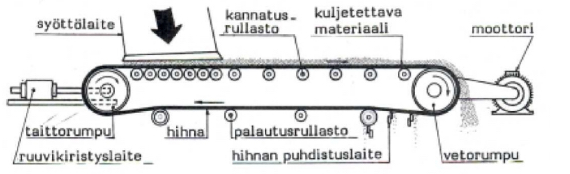
\includegraphics[scale=0.75]{hihnakuljetin_rakenne}
	\end{center}
	\caption{Hihnakuljettimen perusrakenne.
		\cite{Ruokolainen}}
	\label{fig:hihnakuljetin_rakenne}
\end{figure}

\noindent
Hihnakuljettimien alkuinvestointi on melko suuri, mutta käyttökustannukset ovat pienet ja toimintavarmuus hyvä \cite{Hakapää}.Hihnakuljetuksen etuja ovat myös tasainen malmivirta jatkokäsittelyyn ja täysi sähkökäyttöisyys, mikä vähentää tuuletuksen tarvetta maanalaisissa kaivoksissa verrattuna dieselkäyttöiseen malminsiirtoon. Hihnakuljetinta pyörittäviltä sähkömoottoreilta vaaditaan tasaista momentin ja pyörimisnopeuden säilyttämistä, jotta hihna ja muut järjestelmän komponentit kuluvat mahdollisimman vähän \cite{MyyntiHaastattelu}. Tuotannon vaihtelusta johtuen moottorille aiheutuva kokonaiskuorma voi vaihdella ajoittain, mutta äkillisiä kuormanvaihteluita ei pääse juuri syntymään hihnan rajallisen syöttökapasiteetin vuoksi. Kuvassa ~\ref{fig:conveyor} nähdään kalkkikivikaivoksella malmin siirtoon käytetty hihnakuljetin.

\begin{figure}[H]
	\begin{center}
	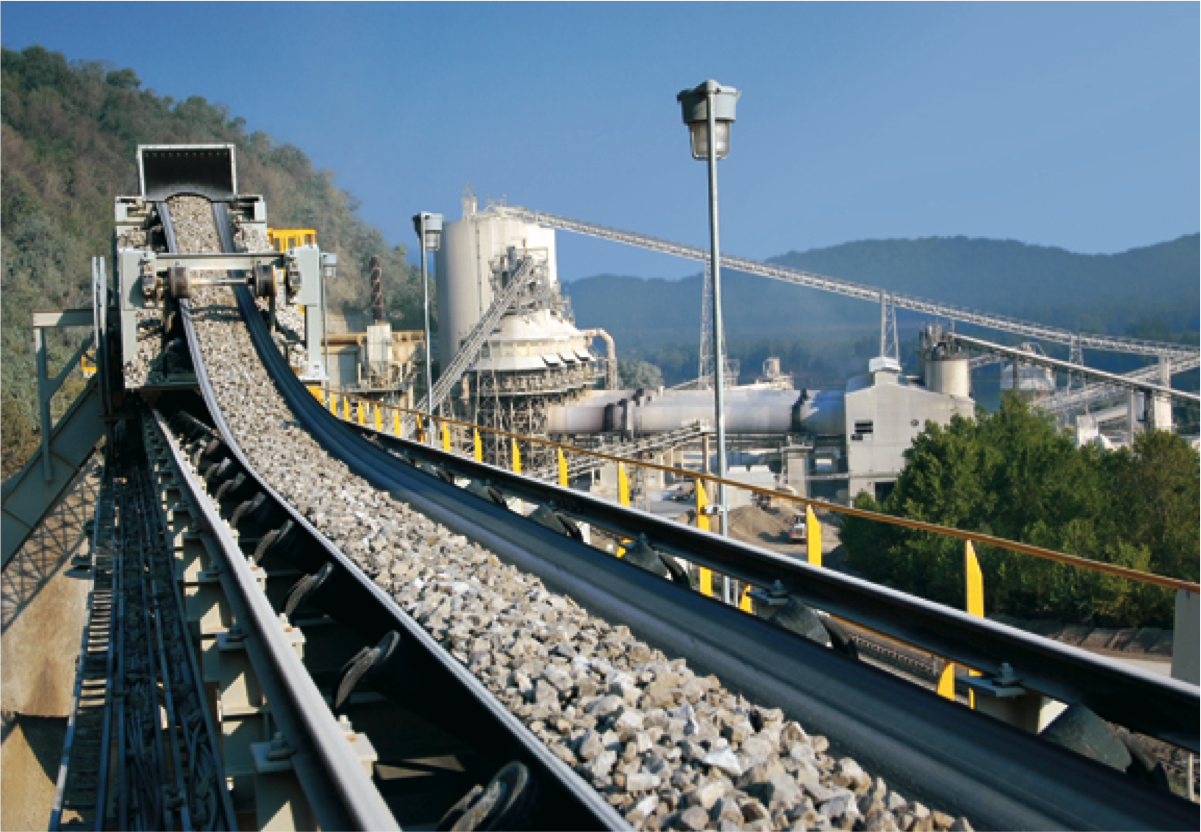
\includegraphics[scale=0.6]{conveyor}
	\end{center}
	\caption{Hihnakuljetin.
		\cite{conveyor}}
	\label{fig:conveyor}
\end{figure}

\noindent
Hihnakuljettimet on perinteisesti varustettu sähkömoottorilla, joka on vaihteiston välityksellä kytketty vetorumpuun. Tällöin kuljetin pystytään ainoastaan kytkemään päälle ja pois, ja sen päällä ollessa ajamaan vain vakionopeudella. Ohjaamattoman sähkömoottorin kytkeminen suureen kuormaan kuten valmiiksi täyteen kuljettimeen aiheuttaa suuret niin mekaaniset kuin sähköiset rasitukset kuljettimen rakenteelle. Kuljettimen vaatima momentti liikkeelle lähtiessä on lisäksi lepokitkan vaikutuksen takia huomattavan suuri, mikä aiheuttaa moottorissa hyvin suuren virrantarpeen. Tämä voi kaivoksesta riippuen aiheuttaa häiriöitä koko sähköverkon toiminnassa.\cite{MyyntiHaastattelu}
\\\\
Tätä käynnistysprosessia voidaan tehdä tehokkaammaksi ja laitteiston kannalta ystävällisemmäksi käyttämällä taajuusmuuttajaa. Kuten aikaisemmin kappaleessa 2.1 todettiin, taajuusmuuttajalla pystytään tuottamaan huomattavasti moottorin ominaismomenttia suurempi vääntö hitailla nopeuksilla. Tämän lisäksi taajuusmuuttajalla on mahdollista käyttää hyvinkin pitkää ramppikäynnistysaikaa, mikä kiihdyttää kuljettimen hitaasti haluttuun nopeuteen. Myös turvallisuusjärjestelmä on edullisempi toteuttaa kun hintavien kontaktoreiden sijaan voidaan käyttää STO-toimintoa. 
\\\\
Hihnakuljettimiin yhdistetyillä taajuusmuuttajilla voidaan lisäksi saavuttaa säästöjä ja tuottaa sähköä, jos käytetään verkkoon jarruttavia taajuusmuuttajia. Jos malmin siirto on alamäkeen, joudutaan hihnan pyörimistä hidastamaan. Tämä on perinteisesti tehty mekaanisen jarrun avulla, missä malmin liike-energia on mennyt hukkaan. Verkkoon jarruttavalla taajuusmuuttajalla voidaan kaivoksen sähköverkkoon tuottaa energiaa malmin potentiaalienergiasta. Espanjassa on toteutettu liukuhihnan jarrutusenergian talteen ottava järjestelmä, joka nyt tuottaa kaivoksen sähköverkkoon 15 megawatin tehon \cite{Rodriguez}.
\\\\
Taajuusmuuttajien käyttö kuljettimien ohjaukseen on yksinkertaista toteuttaa ja  niiden käyttö tuo useita hyötyjä. Tapauksesta riippuen niiden vaatimat investoinnit voivat kuitenkin rajoittaa käyttöönottoa. Yksikertaisissa sovelluksissa, missä kuljettimen pituus on pieni, voi taajuusmuuttajan lisäämisestä saatava hyöty olla liian pieni tarvittavaan investointiin verrattuna. 


%-Millaisia erilaisia? (liukuhihnat,ruuvit,nostimet,yms.)\\
%-Nykyratkaisut?\\
%-Miten tamuja hyödynnetään? edut perinteiseen verrattuna?



\subsubsection{Murskaimet ja syöttimet} %ja sekoittimet?
Murskaimet ovat laitteita, joilla louheen raekokoa pienennetään rikastusta varten. Louheen murskaus tapahtuu yleensä useassa osassa, raekoon pienentyessä noin kuudennekseen murskausvaiheiden välillä. Murskaamo koostuu itse murskaimesta ja siihen louhetta syöttävästä syöttimestä. Murskaimet ovat suuria, paljon energiaa käyttäviä laitteita, jotka saavat voimansa suurista sähkömoottoreista. Syöttimen tehtävä on annostella murskaimeen sopiva määrä louhetta kerrallaan, jotta murskain ei tukkeudu.
\\\\
Murskaus voi perustua iskuun tai puristukseen. Molemmille tyypeille on ominaista, että sähkömoottoreista saatavalla pyörivällä liikkeellä kiviainesta joko puristetaan murskaimen osien välissä tai kiviin kohdistetaan voimakas isku pyörivän terän avulla. Leuka-, kierto-, heiluri-, ja karamurskaimet ovat esimerkkejä puristavasta murskaimesta ja iskupalkkimurskaimet iskuperiaatteella toimivasta.
\\\\
Taajuusmuuttajalla murskaimen pyörimisnopeutta voidaan reaaliaikaisesti säätää, mikä vaikuttaa suoraan syntyvän kiviaineksen ominaisuuksiin \cite{Hulthen}. Aikaisemmin jos pyörimisnopeutta on haluttu muuttaa, on täytynyt murksain pysäyttää ja välitystä moottorin ja murskainosan välillä vaihtaa. Myös murskainosien kulumisesta aiheutuu muutoksia murskatun kiviaineksen laatuun, mitä täytyy kompensoida pyörimisnopeutta tai murskaimen halkaisijaa muuttamalla. Taajuusmuuttajalla tämä kompensointi voidaan tehdä reaaliaikaisesti. Hulthenin tutkimuksessa \cite{Hulthen} taajuusmuuttajalla ohjatun kartiomurskaimen pyörimisnopeutta säädettiin automaattisesti perustuen massavirta-antureilta saatuun dataan. Tällä menetelmällä saavutettiin 15\% kasvu murskaimen kapasiteetissa.
\\\\
Itse murskaimen lisäksi murskaamoon kuuluu joukko murskaimelle louhetta syöttäviä laitteita. Näihin kuuluvat kuljettimet ja syöttimet. Moderneissa murskaimissa kaikkia toimintoja ohjataan keskitetysti ohjaamosta. Käynnistyssykli on yleensä automaattinen logiikan hoitaessa koneen komponenttien oikean käynnistysjärjestyksen. Taajuusmuuttajilla moottoreiden ohjaaminen helpottuu ja esimerkiksi ramppikäynnistyksiä voidaan käyttää vähentämään mekaanista rasitusta.

%\subsubsection{Hissit}
%-Tarvitseeko tälle oman kappaleen?
%-Henkilöhissit, junat, kärryt. Millä ihmiset liikkuu?

\subsubsection{Ilmanvaihto}
Maanalaisissa kaivoksissa koneellinen tuuletus on välttämätöntä. Tuuletuksen tarpeen luovat koneiden pakokaasut, räjähdyskaasut, pöly, kallioperästä tulevat kaasut kuten radon ja eri työvaiheet kuten poraus \cite[s. 290]{Hakapää}. Näistä merkittävin ilmanlaatua huonontava tekijä ovat dieselkoneiden aiheuttamat pakokaasut ja pienpartikkelit \cite[s. 290]{Hakapää}. Jotta työntekijöiden hyvinvointi ja turvallisuus voidaan taata, on laissa määritelty kaivoksen tuuletussuunnittelua ja ilmanlaatumittauksia koskevia asioita \cite[s. 285]{Hakapää}.
\\\\
Kaivoksen tuuletusjärjestelmä perustuu joko alipaineiseen, ylipaineiseen tai molempia käyttävään ratkaisuun. Ali- tai ylipaine luodaan kaivokseen suurilla maanpäällisiällä pääpuhaltimilla, jotka siis joko imevät ilmaa kaivoksesta tai puhaltavat ilmaa sisään. Imevässä tapauksessa korvausilma tulee kaivokseen erikseen louhittua tai muuten avointa reittiä pitkin. Pääpuhaltimien lisäksi paikallistuuletuksella ilmaa ohjataan esimerkiksi louhittaviin periin, missä ilman läpiveto ei ole mahdollista. Lisäksi pääpuhaltimilta tuleva ilma täytyy ohjata tehokkaasti kaivoksen sisällä estäen esimerkiksi likaisen ja puhtaan ilman sekoittuminen matkan varrella. Tämä saadaan aikaan puhaltimilla, seinillä, säleiköillä tai kylmäilmaverhoilla.
\\\\
Puhaltimien liikuttamaa ilmamäärää on perinteisesti ohjattu rajoittamalla ilman kulkua tai mekaanisesti puhallinlapojen kulmaa säätämällä. Lisäksi kaivoksessa olevat ilmanohjaimet kuten seinät ja säleiköt ovat mekaanisesti säädettäviä, jotta kaivoksen tuuletusta pystytään säätämään olosuhteiden muuttuessa. Automaation yleistyessä, on alettu ottaa käyttöön automaatiojärjestelmiä tuulettimien ohjauksessa. Näin on mahdollista luoda reaaliajassa säätyvä tuuletusjärjestelmä, joka mittaa kaivoksen ilmanlaatua ja säätää tuuletuksen tehoa sen mukaan. Kaivosilmasta voidaan mitata esimerkiksi kosteutta, lämpötilaa ja pölypitoisuutta.
\\\\
Kuten luvun 2 alussa mainittiin moottorinohjaus kuristamalla on energiankulutuksen kannalta hyvin epätehokasta. Taajuusmuuttajalla ohjattua puhallinta pystytään reaaliajassa säätämään, niin että haluttu ilmamäärä saavutetaan. Taajuusmuuttaja on oivallinen työkalu paikalliseen tuuletuksen automatisointiin, jossa taajuusmuuttaja ohjaa yhtä tuuletinta esimerkiksi lämpöanturilta saatavan datan mukaan. Taajuusmuuttaja on hyödyllinen myös osana laajempaa automaatiojärjestelmää, jossa PLC lähettää puhaltimen ohjaussignaalin taajuusmuuttajalle esimerkiksi kenttäväylää hyödyntäen. Kenttäväyliä hyödyntämällä kaapeloinnin määrä vähenee huomattavasti ja etenkin kaivoksissa, missä vetomatkat voivat olla kilometrejä, tuovat huomattavia säästöjä. Myös turvallisuuslogiikan integrointi kenttäväylään esimerkiksi PROFIsafella vähentää tarvittavan kaapeloinnin määrää.
\\\\
Kittilän kultakaivoksella puhallinautomaatio on rakennettu käyttäen ABB:n ACS880 taajuusmuuttajia yhdistettynä ABB:n valmistamaan logiikkaohjaimeen. Sen tuomat hyödyt liittyvät saatuihin kustannusetuihin, jotka on saatu käyttämällä vain yhtä kenttäväyläkaapelia ohjaus- ja monitorointitiedon siirtämiseen. Kenttäväylää hyödyntämällä on mahdollista päästä etäältä käsiksi yksittäisten taajuusmuuttajien parametreihin. Tämä vähentää myös henkilöstökuluja, koska yksi operaattori voi säätää koko järjestelmää ilman tarvetta mennä itse toimilaitteen luokse.
%Tähän vielä kittiläkalvoista jotain. Pyydä petriltä

%-Varajärjestelmät?

\subsubsection{Pumput}
Kaivoksiin kertyy vettä ympäristön asettamista syistä kuten pohjavesien valumista ja paikallisista sääolosuhteista johtuen. Lisäksi kaivosprosessin eri vaiheet kuten pölyn sidonta ja poraaminen vaativat vettä, joka tuodaan kaivokseen putkistoa pitkin vesijohtoverkosta tai esimerkiksi läheisestä järvestä. Tätä kaivokseen kertyvää vesimassaa täytyy jatkuvasti pumpata ylös kaivoksesta, jotta kaivos ei tulvi. Kaivoksessa erityisen haasteen pumppaamiselle aiheuttaa veden seassa oleva kiinteä aines. Kiinteä aines täytyy saostaa pois vedestä kaivoksen sisällä ennen pumppaamista, jotta nestemäiselle aineelle tarkoitetut pumput eivät tukkiudu tai vaurioidu. Pumppaus on myös mahdollista tehdä siihen suunnitelluilla lietepumpuilla, jolloin saostusta ei tarvita. Saostus tapahtuu sille rakennetuissa saostusaltaissa, joista pumput pumppaavat puhdistunutta vettä pois.
\\\\
Pumppuilla ohjataan pääsääntöisesti painetta, virtausnopeutta tai säiliön pinnankorkeutta. Pumppujen ohjaus on perinteisesti toteutettu anturilla, joka kytkee pumpun päälle kun tietty raja-arvo ylitetään ja pois kun se taas alitetaan. \cite{Hakapää}. Ratkaisu on hyvin yksinkertainen, mutta energiankulutus on suurta, sillä pumppua käytetään yleensä kaukana optimaaliselta toiminta-alueelta. Kaksiarvoinen pumpun ohjaus aiheuttaa myös äkillisiä paineenvaihteluita putkistoon, mikä aiheuttaa rasituksia itse pumpulle ja putkistolle.
\\\\
Taajuusmuuttajilla pumppuja pystytään muiden sovellusten tapaan ohjaamaan portaattomasti. Painetta, virtausnopeutta tai pinnankorkeutta voidaan ohjata takaisinkytkennällä käyttäen PID-säätöä, jolloin prosessiarvon, esimerkiksi paineen, heilahtelut pienenevät huomattavasti. Sovelluskohtaisella ohjelmistolla varustetut ABB:n ACQ810 taajuumuuttajat pystyvät arvioimaan virtausta myös ilman virtaus- tai painesensoreita, mikä vähentää käyttöönottokuluja tilanteissa, joissa suurta tarkkuutta ei tarvita [ACQ810 esitelähde]. Ohjelmistossa on myös automaattisia toimintoja kuten pumpun puhdistus, joka puhdistaa pumpun nopeilla suunnanvaihdoksilla käyttäjän toimesta tai määräajoin. [ACQ810 esitelähde] Kuten luvussa 1 mainittiin, taajuusmuuttaja mahdollistaa helpon prosessiarvon etäohjauksen ja -valvonnan, sekä turvallisuustoiminnot esimerkiksi kenttäväylää hyödyntäen.
\\\\
Taajuusmuuttajien tuoma uusi pumppusovellus on rinnankytkettyjen puppujen ohjaaminen energiatehokkaalla ja pumppuja vähiten rasittavalla tavalla. Useampi taajuusmuuttaja kommunikoin tällöin keskenään säätäen jokaisen pumpun toiminnan mahdollisimman lähelle optimaalista toimintapistettä, pitäen samalla ohjatun prosessiarvon halutulla tasolla. Pumppuvian ilmetessä taajuusmuuttajat automaattisesti kytkevät kyseisen pumpun pois päältä ja jatkavat toimintaa jäljellä olevilla pumpuilla. 
\\\\
Kaivoksissa pumpun toiminta perustuu useimmiten pinnankorkeuden säätelyyn, pumppujen tarkoituksen ollessa vain veden poistaminen kaivoksen sisältä esimerkiksi saostusaltaasta. Tällöin pumpulta vaaditaan kestävyyttä pumpattavan nesteen ollessa usein kiintoainepitoista ja mahdollisesti hapanta. Tällöin taajuusmuuttajalla ohjattu pumppu on hyödyksi seurattaessa pumpun tilaa etenkin lietepumppauksessa, missä pumpun joutuvat hyvin kovalle rasitukselle. Taajuusmuuttajalla kyetään pumppua valvomaan etäältä ja tarvittaessa tehdä esimerkiksi puhdistustoiminto, jos pumpun kapasiteetin huomataan laskeneen. Pumpattaessa puhdasta vettä esimerkiksi porausyksiköille on ohjattavana suureena porausyksikön vedenpaine, minkä halutaan pysyvän vakiona. Tällöin vaaditaan jatkuvaa takaisinkytkettyä ohjausta, mihin vaaditaan nopeasti paineen vaihteluun reagoiva pumppu. Taajuusmuuttajalla tämä pystytään toteuttamaan yksinkertaisesti taajuusmuuttajan PID-säätimellä.

\subsubsection{Kompressorit}
Moderneissa kallioporakoneissa hydrauliset järjestelmät ovat pääosin korvanneet paineilmaa voimanlähteenään käyttäneet koneet\cite[s. 143]{Hakapää}. Paineilmalla on kuitenkin edelleen rooli joissakin porasovelluksissa, ruiskubetonoinnissa ja räjähdysaineen panostuksessa. Paineilmaa verten kaivoksiin on yleensä rakennettu ruostumattomasta teräksestä valmistettu paineilmaverkosto, johon syöttävät ilmaa omaan tilaansa asennetut kompressorit\cite[s. 269]{Hakapää}.
\\\\
Pumppujen tapaan paineilmaa voidaan tuottaa kompressorilla, joka siirtyy kevennetylle käynnille kun saavutetaan tietty painetaso. Toinen vaihtoehto on käyttää muuttuvanopeuksista kompressoria, joka säätää pyörimisnopeuttansa jatkuvasti vastaten sen hetkiseen painetarpeeseen putkistossa. \cite[s. 269]{Hakapää}. Sovelluksesta riippuen muuttuvanopeuksinen kompressori voi säästää paljon energiaa, mutta esimerkiksi tapauksissa joissa paineen tarve on lähes vakio, on tavallinen kompressori hyötysuhteeltaan yleensä parempi.
\\\\
Kuten pumppusovelluksissa, useita kompressoreita käsittävä järjestelmä on myös mahdollinen. Tällöin ulkoinen teollisuus-PC tai keskenään kommunikoivat taajuusmuuttajat ohjaavat samaan putkistoon kytkettyjä kompressoreita. Tämä mahdollistaa myös erilaisten kompressorien käytön samassa systeemissä. Paineilmasovelluksissa onkin yleistä, että yhden suuritehoisen kompressorin sijaan käytetään muutamaa suurta peruskuormituskonetta ja muutamaa pienempää huippukuormituskonetta, jotka aktivoidaan vain painetarpeen vaatiessa.
\clearpage

\section{Yhteenveto}
%Toiminnallisuus
Tutkimuksen aiheina olivat taajuusmuuttajien sisäisen toiminnallisuuden nykytilanne, niiden rakenne ja kestävyys kaivosolosuhteissa sekä taajuusmuuttajista saatava hyöty kaivosten prosesseissa. Toiminnallisuuden tarkastelussa huomattiin, että taajuusmuuttajat ovat viime vuosina kehittyneet yhä enemmän itsenäisiksi prosessilaitteikseen, joissa kyetään suorittamaan laskentaa ja ohjaamaan moottorin lisäksi myös muita laitteita I/O:ta tai kenttäväylää käyttäen. Kenttäväylien tuomat edut verrattuna perinteisiin analogi- tai digitaalisignaaleihin on saanut myös kaivosteollisuuden toimijat toteuttamaan kenttäväyliä käyttäviä automaatiojärjestelmiä kaivosympäristöön. Työntekijöiden turvallisuus ja yhä tiukkenevat turvallisuusmääräykset ovat saaneet taajuusmuuttajavalmistajat toteuttamaan turvallisuustoimintoja taajuusmuuttajiin, tämä laskee turvallisuuslaitteiston kuluja ja on näin houkutteleva ominaisuus teollisuuden toimijoille.
\\\\
%Kaivosympäristö
Kaivos on haastava ympäristö kaikille koneille, mutta erityisesti elektroniikkalaitteille, koska ne ovat herkkiä niin kosteudelle kuin pölylle. Kaivosympäristössä kosteus, tärinä, pöly ja muut korroosiota aiheuttavat tekijät aiheuttavat taajuusmuuttajat jäähdytysjärjestelmän tehon heikkenemistä ja pahimmassa tapauksessa myös sähköisiä vikoja ja jopa läpilyönnin piirilevyllä. Haastavia ympäristöoloja vastaan taajuusmuuttajavalmistajat ovat tuoneet markkinoille erilaisilla kotelointiratkaisuilla varustettuja taajuusmuuttajia. Niiden kestävyys vaihtelee sisäkäyttöön suunnitelluista avoimista laitteista lähes vesitiiviisiin. Kaivoksen ominaisuuksista riippuen erilaisia kotelointeja käytetään, mutta tutkimuksessa selvisi, että edes suurimmalla kotelointiluokalla varustetut taajuusmuuttajat eivät välttämättä selviydy tietyn tyyppisten kaivosten syövyttävistä ja kosteista ympäristöoloista. Näissä tapauksessa herkkä tehoelektroniikka on asennettuna omaan eristettyyn sähkötilaansa, joiden ilman ominaisuudet ovat sisätiloja vastaavat. Koska sähkötilat ovat keskitettyjä, voivat moottorikaapelien pituudet olla kaivoksissa huomattavan pitkiä. Tämä tulee ottaa huomioon taajuusmuuttajan ominaisuuksia suunniteltaessa. 
\\\\
%Sovellukset
Taajuusmuuttajien potentiaaliset sovellukset ulottuvat kaivosteollisuudessa kaikkialle, missä sähkömoottoreita käytetään. Tällöin taajuusmuuttajien käyttö perustellaan joko energiansäästöllä tai parantuneella kyvyllä ohjata kyseessä olevaa prosessia. Energiansäästö perustuu taajuusmuuttajan kykyyn ohjata suoraan sähkömoottorin tehoa pyörimisnopeuden ja momentin avulla. Tämä on sovelluksesta riippuen huomattavasti energiatehokkaampaa kuin esimerkiksi nopeuden säätäminen jarrun avulla. Etenkin prosesseissa, missä nopeutta joudutaan jatkuvasti muuttamaan tuovat taajuusmuuttajat suuria energiasäästöjä perinteiseen ratkaisuun verrattuna. Energiasäästöjen lisäksi taajuusmuuttajat voivat investointikustannuksestaan huolimatta tuoda säästöjä myös asennuksessa, kun vaihteistojen, kontaktoreiden ja turvalogiikoiden tarve vähenee. Taajuusmuuttajilla saavutetut parannukset prosessin ohjauksessa voivat myös olla ratkaiseva syy niiden käyttöönotossa. Esimerkiksi pumppujärjestelmien älykäs ohjaus ja kuljettimien ramppikäynnistys ovat sovelluksia, joissa älykkäällä toiminnallisuudella saavutetaan epäsuoria säästöjä esimerkiksi vähentyneenä laitteiston kulumana ja parantuneena prosessin tehokkuutena.
\\\\
%Lopetus
Kirjallisten lähteiden, haastatteluiden ja yritysvierailun perusteella on ilmeistä, että taajuusmuuttajilla on lukuisia käyttömahdollisuuksia kaivosteollisuuden alalla. Tekniikan kehitys ja tietoisuus energiankulutuksesta ja ympäristöasioista kiihdyttävät perinteisten ohjausmenetelmien korvaamista  taajuusmuuttajilla. Kaivoteollisuus on pitkään ollut automaatioasteeltaan jäljessä muita suuria teollisuudenaloja, mutta älykkäiden hajautettujen automaatiojärjestelmien kehittyessä on automaation taso, ja samalla taajuusmuuttajien käyttö, kaivoksissa kasvanut. Tulevaisuudessa sähkömoottoreiden yhä enemmissä määrin korvatessa polttomoottorit, on taajuusmuuttajille yhä suurempi tarve, kun tarvitaan tehokasta ja tarkkaa moottorisäätöä.


%-Energiansäästö\\
%-Kustannukset\\
%-Tarkemmat prosessit\\
%-Tulevaisuus?
%-->profit

%\section{Summary} 

\clearpage

%% Lähdeluettelo
\thesisbibliography
\begin{thebibliography}{99}
	
\bibitem{maanlampo}Fridleifsson, Ingvar B., Bertani, Ruggero, Huenges, Ernst, Lund, John W., Ragnarsson, Arni ja Rybach, Ladislaus. \textit{The possible role and contribution of geothermal energy to the mitigation of climate change.} IPCC Scoping Meeting on Renewable Energy Sources. Luebeck, Germany, 2008, Saatavissa: \url{http://www.ipcc.ch/pdf/supporting-material/proc-renewables-lubeck.pdf}

\bibitem{Hakapää}Hakapää,\ A. ja Lappalainen,\ P. \textit{Kaivos- ja louhintatekniikka.} 2.\ painos. Helsinki, Vammalan kirjapaino Oy, 2007.

\bibitem{IP}IEC 60529. \textit{Degrees of protection provided by enclosures (IP Code).} Versio 2.1, Geneve, Sveitsi, International Electrotechnical Commission, 2001.

\bibitem{Rumpunen}Rumpunen, A. \textit{Tuulivoiman vaatimukset taajuusmuuttajalle.} Kandidaatintyö. Aalto-yliopisto. 
Insinööritieteiden korkeakoulu. Espoo. 2012.

\bibitem{ABBtechnicalguide}ABB Drives \textit{Technical guide book}, 2008.

\bibitem{Lukkarinen}Lukkarinen T. \textit{Mineraalitekniikka Osa 1 Mineraalien hienonnus.} Hki: Insinööritieto Oy, 1984.

\bibitem{Anttila}Anttila A. \textit{Kaivosten tuuletusilman energiatehokas lämmitys Suomessa.} Kandidaatintyö. Aalto-yliopisto. Insinööritieteiden korkeakoulu. Espoo. 2014.

\bibitem{Muttilainen}Muttilainen, A. \textit{Lifetime and Reliability of a Frequency Converter’s Fan.} Diplomityö. Aalto-yliopisto. Sähkötekniikan korkeakoulu. Espoo. 2013

\bibitem{Karlsson}Karlsson, S. \textit{Murskaintyyppien ominaisuuksien vertailu}. Kandidaatintyö. Aalto-yliopisto. Insinööritieteiden korkeakoulu. Espoo. 2011.

\bibitem{Hulthen}Erik Hulthén, C. Evertsson, M. \textit{Real-time algorithm for cone crusher control with two variables}. Minerals Engineering.  24. Painos. Numero 9. Elokuu 2011. s. 987-994. Saatavissa: \url{http://dx.doi.org/10.1016/j.mineng.2011.04.007}.

\bibitem{Pyhäsalmi}CUPP, \textit{Pyhäsalmen kaivos.} Verkkodokumentti. Päivitetty 26.3.2013. Viitattu 6.10.2014. Saatavissa: \url{http://www.cupp.fi/index.php?option=com_content&view=article&id=3&Itemid=41&lang=fi	}

\bibitem{ABBinmining}ABB Oy. \textit{ABB drives in mining}. Päivitetty 2012. Viitattu 6.10.2014. Saatavissa: \url{http://www05.abb.com/global/scot/scot216.nsf/veritydisplay/2205e72865c2c747c1257a620026d001/$file/Mining%20brochure_EN_lowres.pdf}

\bibitem{manchao}Man-chao, H. \textit{Application of HEMS cooling technology in deep mine heat hazard control}. Mining Science and Technology (China). 19. Painos, Numero 3. Toukokuu 2009. S. 269-275. Saatavissa: \url{http://dx.doi.org/10.1016/S1674-5264(09)60051-X}.

\bibitem{880hwman}ABB Oy. 2012. \textit{Laiteopas, ACS880-01-taajuusmuuttajat, Rev E}. Saatavissa: \url{http://www05.abb.com/global/scot/scot201.nsf/veritydisplay/71ce8071e2a7ae2bc1257bd70046ade1/$file/FI_ACS880-01_0_55to250kW_HW_E_plus_update_notice_screen.pdf}. Päivitetty 29.6.2012. Viitattu 9.10.2014.

\bibitem{Pallasmaa}Pallasmaa, A. \textit{Ulkokäyttöön Tarkoitetun Tehoelektroniikkalaitteen Konseptisuunnittelu}. Diplomityö. Teknillinen korkeakoulu. Espoo. 2009.

\bibitem{Hartman}Hartman, H. Mutmansky, J. Ramani, R. Wang, Y. \textit{Mine Venilation and Air Conditioning}. New York, Yhdysvallat. John Wiley \& Sons Inc. 1997.

\bibitem{Sirkko}Louhintatyöstä syntyvän tärinän riskiarviointi. Saatavissa: http://www.theseus.fi/handle/10024/42462

\bibitem{danfoss} Saatavissa: \url{http://www.danfoss.com/NR/rdonlyres/2270DF18-D4AD-4808-824E-4942B247F078/0/2011_AutomationDrive_176R0571_Web.pdf}

\bibitem{IEC60082-2}IEC 60082-2. \textit{Environmental testing - Part 2-6: Tests - Test Fc: Vibration (sinusoidal)}. 7.painos. Geneve, Sveitsi. IEC. 2007. 86 s.

\bibitem{MyyntiHaastattelu}Antti Hedman. Myyntipäällikkö. ABB Oy. Haastattelu. 17.10.2014. Pitäjänmäki, Helsinki.

\bibitem{STOkuva}Siemens AG. \textit{Safe Torque Off (STO)}. Saatavissa: \url{http://www.industry.siemens.com/topics/global/en/safety-integrated/machine-safety/product-portfolio/drive-technology/safety-functions/pages/safe-torque-off.aspx}. Päivitetty 10.3.2014. Viitattu 27.10.2014.

\bibitem{SS1kuva}Siemens AG. \textit{Safe Stop 1 (SS1)}. Saatavissa: \url{http://www.industry.siemens.com/topics/global/en/safety-integrated/machine-safety/product-portfolio/drive-technology/safety-functions/Pages/safe-stop1.aspx}. Päivitetty 10.3.2014. Viitattu 27.10.2014.

\bibitem{Profisafe} PROFIBUS \& PROFINET International (PI). \textit{PROFIsafe}. \url{http://www.profibus.com/technology/profisafe/}Päivitetty 10.3.2014. Viitattu 27.10.2014.

\bibitem{FSO} ABB Oy. \textit{User's manual: FSO-12 Safety functions module}. \url{http://www05.abb.com/global/scot/scot201.nsf/veritydisplay/80fd1fe025d402d7c1257d0000408aa6/$file/EN_FSO_12_UM_A_A5.pdf}. Päivitetty 26.3.2014. Viitattu 27.10.2014.

\bibitem{acs880panel}ABB Oy. \textit{ACS880 Control Panel}. Kuva. Saatavissa: \url{http://www04.abb.com/global/seitp/seitp202.nsf/0/2996a31f6d99e961c1257864004ae0c1/$file/HM2011-02b.jpg}. Viitattu 28.10.2014

\bibitem{VSI}Joensuu, T. Eronen, T \textit{Taajuusmuuttajan ohjauksen suunnittelu}. Insinöörityö. Metropolia Ammattikorkeakoulu. 2013. Saatavissa: \url{http://www.theseus.fi/bitstream/handle/10024/67121/Taajuusmuuttajan_ohjauksen_suunnittelu.pdf?sequence=1}. 

\bibitem{Ruokolainen}Ruokolainen P. \textit{Louheensiirtomenetelmät suurella louhoksella.} Kandidaatintyö. Aalto-yliopisto. Kemian tekniikan korkeakoulu. Espoo. 2011.

\bibitem{conveyor}Carmeuse Lime \& Rock. Kuva. Saatavissa: \url{http://www.carmeuseky.com/wp-content/uploads/2012/07/conveyor.png}. Viitattu 9.11.2014

\bibitem{Rodriguez}Rodriguez, J. Pontt, J. Becker, N. Weinstein, A. \textit{Regenerative drives in the megawatt range for high-performance downhill belt conveyors}. Industry Applications. IEEE Transactions painos.38, numero 1. s. 203-210. 2002.

\bibitem{Kaivosprosessi}opasnet.org. Kuva. Saatavissa: \url{http://fi.opasnet.org/fi/Tiedosto:Kaivostoiminnanyleisprosessi.png}. Päivitetty 11.2.2012. Viitattu 12.11.2014.

\bibitem{Brown}Brown, G.M. Elbacher, B.J. Koellner, W.G. \textit{Increased productivity with AC drives for mining excavators and haul trucks}. Industry Applications Conference, 2000. Conference Record of the 2000 IEEE painos.1. s.28,37. 2000.

\bibitem{LHD}Sandvik Oy. \textit{Ground-breaking Electricity}. Saatavissa \url{minestories.com/ground-breaking-electricity}. Päivitetty 2014. Viitattu 12.11.2014

\end{thebibliography}



%% Liitteet
\clearpage

\thesisappendix
\section{Liite 1: Kotelointiluokitus standardin SFS-EN 60529 mukaan\label{Liite 1}}
EN 60529 -standardin mukaisen IP-koodin ensimmäisen tunnusnumeron merkitys
\\\\
\tabulinesep=5pt
\begin{tabu} to \textwidth {|X[2,c]|X[3c]|X[3c]|} 
   \hline
   \rowfont[c]\bfseries %will apply the \bfseries command to all elements of the next row
	Ensimmäinen tunnusnumero & Suojaus vaarallisten osien kosketukselta	 & Suojaus vierailta esineiltä ja pölyltä \\ \hline
    0                        & Suojaamaton                               & Suojaamaton                            \\ \hline
    1                        & Kosketussuojattu nyrkiltä                 & Halkaisijaltaan yli 50 mm esineiltä    \\ \hline
    2                        & Sormelta                                  & Halkaisijaltaan yli 12,5 mm esineiltä  \\ \hline
    3                        & Työkalulta                                & Halkaisijaltaan yli 2,5 mm esineiltä   \\ \hline
    4                        & Langalta                                  & Halkaisijaltaan yli 1 mm esineiltä     \\ \hline
    5                        & Langalta                                  & Pölysuojattu                           \\ \hline
    6                        & Langalta                                  & Pölytiivis                             \\ \hline

\end{tabu}
\\\\
\\\\
\\\\
EN 60529 -standardin mukaisen IP-koodin toisen tunnusnumeron merkitys
\\\\
\tabulinesep=5pt
\begin{tabu} to \textwidth {|X[2,c]|X[6,c]|} 
   \hline
   \rowfont[c]\bfseries %will apply the \bfseries command to all elements of the next row
	Toinen tunnusnumero      & Vesisuojaus															\\ \hline
    0                        & Suojaamaton                           								\\ \hline    
    1                        & Suojattu pystysuoraan tippuvalta vedeltä                				\\ \hline
    2                        & Suojattu korkeintaan 15 asteen kulmassa tippuvalta vedeltä 			\\ \hline
    3                        & Suojattu korkeintaan 60 asteen kulmassa satavalta vedeltä            \\ \hline              
    4                        & Suojattu kaikista suunnista roiskuvalta vedeltä              		\\ \hline              
    5                        & Suojattu kaikista suunnista tulevalta vesisuihkulta                  \\ \hline               
    6                        & Suojattu kaikista suunnista tulevalta voimakkaalta vesisuihkulta		\\ \hline
	7                        & Suojattu lyhytaikaisen veteen upottamisen haittavaikutuksilta		\\ \hline
	8                        & Suojattu jatkuvan veteen upottamisen haittavaikutuksilta 			\\ \hline
\end{tabu}
\end{document}
